\NeedsTeXFormat{LaTeX2e}[2005/12/01]
%%    2010/01/01 v1.7 IMTEK-Diplomarbeitsvorlage
%% Template fuer Diplom-, Bachelor- und Masterarbeiten
%% am IMTEK (c) Simon Dreher
%% Verbesserungsvorschlaege bitte an dreher@imtek.de

%%%%%%%%%%%%%%%%%%%%%%%%%%%%%%%%%%%%%%%%%%%%%%%%%%%%%%%%%%
%%%%%%%%%% Bitte vor dem Veraendern umbenennen! %%%%%%%%%%
%%%%%%%%%%%%%%%%%%%%%%%%%%%%%%%%%%%%%%%%%%%%%%%%%%%%%%%%%%

%% Moegliche Optionen: diejenigen der Klasse scrbook ausser titlepage

%% deutsche DA:
\documentclass[master,         %% Typ der Arbeit: diplom, bachelor oder master
               12pt,           %% Schriftgroesse
               twoside,        %% zweiseitiges Layout
               BCOR10mm,       %% Bindekorrektur 10 mm
%               liststotoc,nomtotoc,bibtotoc, %% Aufnahme der div. Verzeichnisse
                                              %% ins Inhaltsverzeichnis
%               pointlessnumbers, %% Ueberschriftnummer. ohne angehaengtem Punkt
               ngerman,english%% Alternativspr. Englisch, Dokumentspr. Deutsch
%               final,          %% Endversion; draft fuer schnelles Kompilieren
							 ]{IMTEKda}
%% Englisch mit dt. Vorspann:
% \documentclass[diplom,12pt,twoside,BCOR10mm,pointlessnumbers,ngerman,english,noenglishpreamble]{IMTEKda}

%% Labels anzeigen zur Korrektur
%\usepackage{showkeys} %% Labels verschwinden mit der Klassenoption final

\usepackage{babel}     %% Sprachen-Unterstuetzung
\usepackage{calc}      %% ermoeglicht Rechnen mit Laengen und Zaehlern
\usepackage[T1]{fontenc}
\usepackage[latin1]{inputenc}
%% in aktuellem Linux & MacOS X wird standardmaessig UTF8 kodiert!
%\usepackage[utf8]{inputenc}

\usepackage{amsmath,amssymb} %% zusaetzliche Mathe-Symbole

\usepackage{lmodern} %% type1-taugliche CM-Schrift als Variante zur
                     %% "normalen" EC-Schrift
%% Variante: Schriftumschaltung auf URW Garamond und Bitstream Vera
%\usepackage[garamond,sfscaled=false,ttscaled=false]{mathdesign}
%\usepackage[scaled=0.9]{berasans,beramono}

\usepackage{color}
\usepackage{framed}

\usepackage{array}
\newcolumntype{L}[1]{>{\raggedright\let\newline\\\arraybackslash\hspace{0pt}}m{#1}}
\newcolumntype{C}[1]{>{\centering\let\newline\\\arraybackslash\hspace{0pt}}m{#1}}
\newcolumntype{R}[1]{>{\raggedleft\let\newline\\\arraybackslash\hspace{0pt}}m{#1}}


%% Paket fuer bibtex-Datenbanken
\usepackage[comma,numbers,sort&compress]{natbib}
%\usepackage{babelbib}         %% korrekte Sprache in Bibliographieeintraegen
\bibliographystyle{plainnat}  %% Formatierung Bibliographie ohne babelbib
%\bibliographystyle{babplain}  %% Formatierung Bibliographie mit babelbib
\usepackage{varioref}

\newcommand{\tabheadfont}[1]{\textbf{#1}} %% Tabellenkopf in Fett
\usepackage{booktabs}  %% Befehle fuer besseres Tabellenlayout
\usepackage{longtable} %% umbrechbare Tabellen
\usepackage{multirow}
%\usepackage{array}     %% zusaetzliche Spaltenoptionen
%\usepackage{rotating}
\usepackage{pdflscape}

%% umfangreiche Pakete fuer Symbole wie \micro, \ohm, \degree, \celsius etc.
\usepackage{textcomp,gensymb,chemarr,bpchem,float}

%\usepackage{SIunits} %% Korrektes Setzen von Einheiten
\usepackage{units}   %% Variante fuer Einheiten

%\usepackage{icomma}  %% Abstandskorrektur fuer , als Dezimaltrenner

\widowpenalty=10000
\clubpenalty=10000

\usepackage{setspace}
%\onehalfspacing  %% 1,5-facher Zeilenabstand

\usepackage[pdftex]{graphicx}
\usepackage{epstopdf}

%% Hyperlinks im Dokument; muss als eines der letzten Pakete geladen werden
\usepackage[pdfstartview=FitH,      % Oeffnen mit fit width
            breaklinks=true,        % Umbrueche in Links, nur bei pdflatex default
            bookmarksopen=true,     % aufgeklappte Bookmarks
            bookmarksnumbered=true, % Kapitelnummerierung in bookmarks
            pdfprintscaling=None,   % Default-Einstellung zum Drucken: nicht skaliert
            pdfduplex=DuplexFlipLongEdge, % Default-Druck-Einstellung: Duplex
            ]{hyperref}

%% um keine SANSSERIF Schriften fuer Ueberschriften zu verwenden:
%\setkomafont{sectioning}{\normalfont\normalcolor\bfseries}
%% fuer kleinere Bild- und Tabellenunterschriften:
\addtokomafont{caption}{\footnotesize}
\addtokomafont{captionlabel}{\footnotesize\bfseries}
%\addtokomafont{caption}{\footnotesize\sffamily}
%\addtokomafont{captionlabel}{\footnotesize\sffamily\bfseries}

%% um abgekuerzte Abbildungs- und Tabellenbezeichnung mit \autoref zu erhalten:
%\addto{\extrasngerman}{\renewcommand*{\figureautorefname}{Abb.}}
%\addto{\extrasngerman}{\renewcommand*{\tableautorefname}{Tab.}}
\hyphenation{dia-gram}
\hyphenation{fluo-res-cence}
\hyphenation{meas-ure-ment}

%% Erzeugt einen gekreuzten Pfeil
\newlength\pf
\newcommand{\dpf}{
\settowidth\pf{$\nearrow$}
\searrow\kern-\pf\nearrow}

%% Neuer Befehl um die einzelnen Teile a, b, ... eines Bildes zu referenzieren
\newcommand{\sref}[2]{\mbox{\ref{#1}\hspace{1.5pt}#2}} 

\begin{document}

\author{Zhonglei Zhou}
\title{Development of a Novel Modular Reusable and Resealable Microfluidic Platform}
\hypersetup{pdfkeywords={IMTEK, Masterarbeit, master's thesis}}

%% Einfuegen eines Titelbilds (optional)
\titlepic{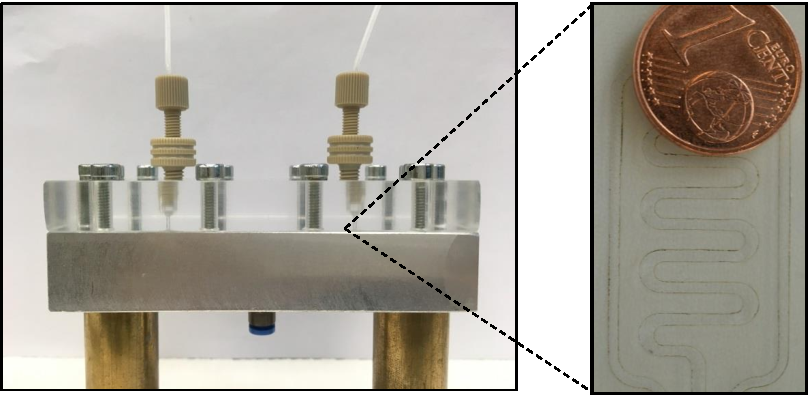
\includegraphics[width=0.9\textwidth]{figures/title}}
\titlepicdesc{The picture shows the integration of the microfluidic platform and one microchannel design}

%% Die jeweils auskommentierte Variante ist bei englischer Praeambel zu verwenden
%\dpoversion{20.\,7.~2001}
\dpoversion{2009}
%\dpoversion{28.\,9.~2000}       %% DPO 2000
%\dpoversion{September 28, 2000} %% DPO 2000
%\chair{Lehrstuhl f"ur \dots}
\chair{Design of Microsystems}
\referees{Prof.\ Dr. Peter Woias,\\ Laboratory for Design of Microsystems\\ \\
Prof. Dr. Ulrike Wallrabe,\\ 
Laboratory for Microactuators}

\supervisor{Dr. Keith Cobry, \\ Laboratory for Design of Microsystems}
%\thesistime{1.\ Januar 2006 bis 31.\ Mai 2006}
\thesistime{May~1, 2016 to April~25, 2017}

\frontmatter
\maketitle
\cleardoublepage\phantomsection\pdfbookmark{\abstractname}{abstract} %% fuegt ersten Abstract in die Bookmarks ein
%\begin{otherlanguage}{ngerman}
\begin{abstract}
This thesis presents the development of a modular reusable and resealable microfluidic platform designed for the future study of near-wall bacteria deposition and adhesion features during filtration processes, which requires the flexibility of creating different predictable hydrodynamic environments. This microfluidic platform is able to operate under high pressure (up to 10bar) and its reusability and resealability allows it to be reassembled for many times as well as providing excellent sealing performance under high pressure. This microfluidic platform is versatile for the integration of different sheets as ``surface samples'' including non-permeable sheet and semipermeable membranes, near which the bacteria adhesion during real filtration processes occurs. The transparent lid of the microfluidic platform provides direct observation into the microchannel during the adhesion process.\\

A novel laser rapid prototyping technique is introduced for the patterning of microchannels in silicone membranes of the thickness of 200$\mu$m. This new technique is able to process microstructures in the silicone membranes with indirect ablation, a sacrificial steel sheet is ablated by the laser and the silicone membrane is then ablated by the ejected metal sputtering and plasma. Through-cut microchannels are realized by this laser rapid prototyping with acceptable processing accuracy and the possibility of machining microchannels with variable depth is also verified. Moreover, high design flexibility is achieved with the use of computer aided design of the microchannel geometry. A glass slide is used as the mechanical carrier of the silicone microchannel and also offers full view of the microchannel. \\

In initial tests, the microchannel was characterized by measuring the cross flow rate of certain channel geometry with respect to the working pressure, with which the pressure drop along the microchannel and its fluidic resistance can be figured out. This indicates that the hydrodynamic conditions inside the microchannel can be studied and controlled for the research into the forces involved with bacteria adhesion. Reusability with commercial nanofiltration membrane samples in the microfluidic platform and its permeability in dead end mode was also characterized with different solutions. The compacting process of the nanofiltration membrane, which is one of the important membrane properties, is observable with current data and matches current theory. Thus we conclude that this microfluidic platform offers the chance for the studying mass transport and deposition/adhesion of bacteria with this microfluidic platform in more detail by further future experiments. \\
  \bigskip\par
  \textbf{Keywords:}  microfluidic platform, high pressure, laser rapid prototyping, nanofiltration membrane.
\end{abstract}
%\end{otherlanguage}
\begin{otherlanguage}{ngerman}
\begin{abstract}
In dieser Masterarbeit wird die Entwicklung einer modularen und wiederverwendbaren mikrofluidischen Plattform f\"ur k\"unftige Studien zur Ablagerung und \\ Fl\"achenadh\"asion von Bakterien in Filtrationsanwendungen vorgestellt. Eine Anforderung an das System ist es, verschiedene vorhersagbare hydrodynamische Umgebungsbedingungen zu schaffen. Die mikrofluidische Plattform muss unter hohem Druck (bis zu 10 bar) betrieben werden k\"onnen und f\"ur das wiederholte Ein- und Ausbauen unterschiedlicher Folien als \glqq Fl\"achenproben\grqq  \ geeignet sein. Nicht permeable sowie semipermeiable Membranen, die in der  Praxis verwendet werden und Bakterienablagerung demonstrieren sollen im System getestet werden k\"onnen. Ein transparenter Deckel erm\"oglicht die direkte Beobachtung des Mikrokanals w\"ahrend der Ablagerungs- und Adh\"asionsprozesse.\\

Ein neuartiges Laser Rapid-Prototyping Verfahren wurde zur Fertigung von \\ Mikrokan\"alen in Silikonfolien (St\"arke 200 $\mu$m) entwickelt. Mit dieser Technik wurden Mikrostrukturen in die, f\"ur den verwendeten Laser transparenten, Silikonmembranen \"uber indirekte Ablation gefertigt. Eine Opferschicht bestehend aus einer Edelstahlfolie wurde als Unterlage bei der Fertigung verwendet. Das Silikon und wurde durch Sputtern des herausgeschleuderten Metalls sowie durch das entstehende Plasma abgetragen. G\"anzlich durchgeschnittene Mikrokan\"ale wurden durch diesen Prozess mit akzeptabler r\"aumlicher Aufl\"osung realisiert. Die Realisierung von verschiedener Strukturtiefen in den Silikonfolien durch diesen indirekten Ablationsprozess wurde ebenfalls gezeigt. Computerunterst\"utztes Design (CAD) erm\"oglicht die rasche/schnelle Entwicklung und Fertigung verschiedenster Kanaldesigns. Die Silikonfolien wurden aufgrund optischer Zug\"anglichkeit auf einfachen Glasstr\"agern gefertigt. \\

In anf\"anglichen Tests des Durchflussbetriebs wurde ein Druckabfall entlang des Kanals gemessen, was zur Ableitung hydrodynamischer Parameter im Kanal f\"uhrt. Eine solche Charakterisierung liefert Daten, die zur Analyse anwesender Kr\"afte w\"ahrend Ablagerung und Adh\"asion genutzt werden k\"onnen. Tests zur Wiederverwendbarkeit und Permeabilit\"at mit Proben einer kommerziell erh\"altlichen Nanofiltrationsmembran wurden durchgef\"uhrt. \"Uber Messungen der Durchflussrate wurde die Verdichtung der Membran, sowie der Betrieb mit Reinstwasser und Salzl\"osungen gepr\"uft. Die Ergebnisse stimmten mit den Erwartungen \"uberein und zeigten gro\ss es Potential f\"ur eine ausf\"uhrlichere Auswertung der Stofftransport- und bakteriellen Ablagerungsprozesse in k\"unftigen Arbeiten.\\
  \bigskip\par
  \textbf{Stichw\"orter:} Mikrofluidische Plattform, Hochdruckbetrieb, Laser Rapid Prototyping, Nanofiltrationsmembran.
\end{abstract}
\end{otherlanguage}

%% fuegt Inhaltsverzeichnis in die Bookmarks ein
\cleardoublepage\phantomsection\pdfbookmark{\contentsname}{toc}
%% setzt Inhaltsverzeichnis
\tableofcontents

\begin{nomenclature}
%% Fuer die Berechnung der Spaltenbreiten muss \usepackage{calc}
%% geladen sein!
\section*{Latin characters}
\noindent
\begin{longtable}[l]{p{0.2\textwidth}p{0.6\textwidth-6\tabcolsep}p{0.2\textwidth}}
  \tabheadfont{Variable}&\tabheadfont{Meaning}&\tabheadfont{Unit}\\\midrule\endhead
	$d$ & depth & $\unit{m}$ \\
	$D$ & diameter & $\unit{m}$\\
	$H$ & height & \unit{m} \\
	$I$ & flow rate & \unit{mL/min} \\
	$l$ & length & \unit{m} \\
	$L$ & permeability & \unit{L/m$^2$hbar} \\
	$p$ & pass & -- \\
	$P$ & pressure & \unit{Pa} \\
	$r$ & radius & \unit{m} \\
	$R$ & fluidic resistance & \unit{Pa$\cdot$ s/m${}^3$} \\
	$R^2$ & coefficient of determination & -- \\
	$V$ & voltage & $\unit{V}$ \\
	$W$ & width & \unit{m} \\
\end{longtable}

\section*{Greek characters}
\begin{longtable}[l]{p{0.2\textwidth}p{0.7\textwidth-6\tabcolsep}p{0.1\textwidth}}
  \tabheadfont{Variable}&\tabheadfont{Meaning}&\tabheadfont{Unit}\\\midrule\endhead
	$\Delta$ & difference & -- \\
    $\eta$ & dynamic viscosity & $\unitfrac{N s}{m^2}$ \\
    $\rho$ & density & $\unitfrac{kg}{m^3}$ \\
\end{longtable}


\section*{Abbrevations}
\begin{longtable}[l]{p{0.2\textwidth}p{0.8\textwidth-4\tabcolsep}}
  \tabheadfont{Abbrevation}&\tabheadfont{Meaning}\\\midrule\endhead
	ADC & analog to digital conveter \\
	BPR & back pressure regulator \\
	CAD & computer-aided design \\
	DAQ & data acquisition \\
	DI & deionized \\
	ETFE & ethylene tetrafluoroethylene \\
    LRP & laser rapid prototyping \\
	LSM & laser scanning microscope\\
	NF & nanofiltration\\
	opamp & operational amplifier\\
	PDMS & polydimethylsiloxane \\
	PEEK & polyether ether ketone\\
	PMMA & poly(methyl methacrylate)\\
	PS & pressure sensor\\
	Re & Reynolds number\\
	RO & reverse osmosis\\
	RP & rapid prototyping\\
	SEM & scanning electron microscope\\
	SS & stainless steel\\
	UF & ultrafiltration\\
	UV & ultraviolet\\	
\end{longtable}
\end{nomenclature}

%% die Klassenoption liststotoc uebernimmt das Abbildungs- und Tabellen-
%% verzeichnis in den TOC
%% \listoftables und \listoffigures sollten nur bei genuegender Anzahl Tabellen
%% verwendet werden
\footnotesize

\listoffigures
\listoftables
\normalsize
\mainmatter   %% Anfang Hauptteil

\chapter{Introduction}
\label{1}
Microfluidic devices have presented an attractive platform to researchers in recent years for performing studies into a wide variety of microbiological processes. Bacteria adhesion, for example, is one of the interested processes to be studied. This thesis project is developed in the framework of microfluidic technology to build a microfluidic platform which may be used for future work studying the bacteria adhesion features at the solid-liquid interfaces. In this chapter the motivation of designing this microfluidic platform and the advantages of this design is discussed. The aim of this thesis work as well as the frame of the thesis will also be explained. Moreover, a brief description of the approach for achieving the goal is presented.

\section{Motivation}
\label{1_1}
The aim of this master thesis work is to design a modular microfluidic platform to study the transport and adhesion mechanism of individual bacteria on both solid and semi-permeable surfaces and their relation to the kinetics and statistics of bacteria deposition in a flow in microfluidic channels. When the bacteria-containing suspension flows in a microchannel, the transported bacteria will either adhere to the wall or slide or roll downstream when it reaches the wall, depending on the surface properties and hydrodynamic conditions. Such adhesion can lead to surface colonization by bacteria and the formation of biofilms (biofilms are sessile microbial communities growing on surfaces). In certain scenarios the growth of these biofilms might be desired at certain locations in a microfluidic system, e.g. for cultivation studies, while in other scenarios this growth can lead to unwanted channel blockage. Therefore the study of such micro-processes is a topic of great interest.\\

When the microchannel is formed by impermeable walls shown in  \autoref{figure1_1} (a), there is only cross flow within the channel. Some studies about the bacteria adhesion feature under such scenario are already done \cite{elimelech2013particle} \cite{levich1962physicochemical}. However, when one side of the wall is replaced by semi-permeable membranes shown in \autoref{figure1_1} (b), the permeate flow is introduced and thus the downstream movement such as sliding and rolling would be affected by the introduced normal drag force. In particular, when the depth of the microchannel varies along its length (\autoref{figure1_2}), the flow velocity will also change along the length of the channel in a single test, leading to the variation of the tangential shear stress. These hydrodynamic variations may provide opportunities to setup a model to study the adhesion mechanism of bacteria at surfaces with different flow rate and multiple flow components.


\begin{figure}[ht]%
\centering
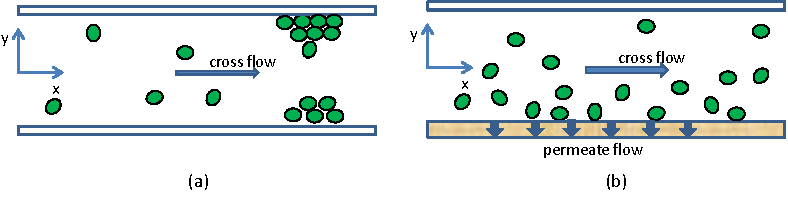
\includegraphics[width=0.8\textwidth]{figures/introduction/figure1_1}%
\caption{(a) Microchannel with impermeable walls. (b) Microchannel with semi-permeable wall on one side.}%
\label{figure1_1}%
\end{figure}

\begin{figure}[ht]%
\centering
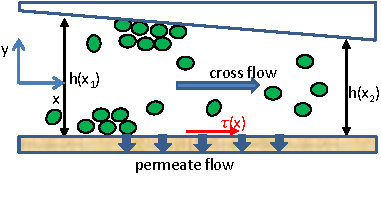
\includegraphics[width=0.4\textwidth]{figures/introduction/figure1_2}%
\caption{Microchannel with variable channel depth.}%
\label{figure1_2}%
\end{figure}

Microfluidic devices, in which low volume of fluids are moved, separated or processed, are now widely used in the research of fluid properties and many kinds of micro-processes in the fluids. On the one hand, the high surface-to-volume ratios in fluids can provide contact area for substance like bacteria to interact with the channel walls, which makes it sometimes easier to obtain measureable and even observable micro-processes such as growing or adhesion of bacteria to the channel walls. On the other hand, small volumes are also easier to be controlled under specific process conditions such as pressure and flow rate. Thus microfluidic devices can provide platforms for generating well-controlled hydrodynamic properties of the flow for studying complex coupled micro-processes in the microchannels. 


\subsection{Microfluidic Platform for Testing of Bacteria Adhesion Features}
\label{1_1_1}
As illustrated in the former section, in this master thesis a microfluidic platform is designed to study the adhesion mechanism of bacteria on both solid and semi-permeable surfaces. The semi-permeable surface in this thesis work is achieved by nanofiltration membranes and the adhesion features of the bacteria during separation are to be studied. This microfluidic platform is supposed to provide an ideal approach for in-depth direct investigation of the microscopic processes that occur at the membrane surface during separations. 

\subsection{Reusable and Resealable for High Pressure Applications}
\label{1_1_2}
Handling fluids at high pressures is quite demanding. Firstly, the forces present must be considered in order to ensure that the structural strength of the device and material is sufficient. Secondly, interfacing and sealing need to be accounted for, usually solved at macro scale by welding and the use of O-rings. Thus it is meaningful and at the same time of great challenge to develop a microfluidic platform for high pressure applications. There are two conventional packaging methods for the housing in high pressure applications, one of which is permanent integrated connections including epoxy gluing, metal soldering or glass brazing \cite{marre2010design}. These connections are able to withstand high pressures in particular designs \cite{blom2001local}. However, such high pressure performance is achieved at the expense of losing the versatility and the reversibility. The non-permanent modular connection methods can also be used for packaging especially for those microfluidic systems which can be assembled and disassembled for multiple times. These connection methods are involved with different kinds of gaskets which can be reused after disassembling and do not hurt the microfluidic system at the same time.\\

In our case, the separation process is achieved by filtering under high pressure with the NF membrane. The pressure will push water molecules through the NF membrane while the charged ions will be repelled by the electrical surface charges on the NF membrane. Bacteria, due to their large physical size, can also not pass through the NF membrane since the mesh size of the NF membrane is within the nanometer range. The deposition and adhesion features of the bacteria are to be studied so that the NF membrane needs to be replaced after a single test by a new piece of NF membrane and this leads to the disassembling and reassembling of the microfluidic platform. Therefore it is of great importance to keep a good sealing performance and steady mechanical stability of the housing after reassembling to make the platform reusable and resealable. 


\subsection{Laser Rapid Prototyping for Flexible Channel Fast Fabrication}
\label{1_1_3}
Rapid prototyping (RP) is a term which embraces a range of new technologies for producing accurate parts directly from three-dimensional computer aided design (CAD) data \cite{pham1998comparison}. This means that the designers have the freedom to produce physical models of their drawings more frequently, allowing them to check the assembly and function of the design. As a result, errors are minimized and the developing cost and lead times are significantly saved. \\

Processing technologies regarding processing microstructures may be divided broadly into those involving the addition of material and those involving its removal \cite{lehmann1995laser}. The main technology for material removal is lithography and etching techniques which can manufacture high quality three-dimensional microstructures. However, these techniques require photo masks to be made before the microstructures can be produced, and the production itself consists of many complicated and time-consuming steps. Besides, any structural redevelopment would require the redesign of the masks. Therefore such techniques are only economical for mass production of a single design that does not need any further development. In the case of this thesis work, however, the design of the microchannel needs to be quite flexible in order to test the filtration features under different channel geometries. As a result, the etching techniques are not the optimal processing techniques with respect to the application in this thesis work.\\

Laser rapid prototyping (LRP) technique developed in this thesis work is defined as laser indirect cut into the work piece. Repeating the laser processing path will simply result in the variation of cutting depth and this gives the possibility for three-dimensional machining. With the use of computer-aided design the structure data could be transferred directly to the laser machine and can be processed within tens of minutes. Therefore high design flexibility can be achieved in this way. Since in this work laser cutting is the only process to fabricate the microchannel and no cleanroom processes and materials are needed, it allows high efficiency of the microchannel design and fabrication and also saves cost significantly. 


\section{Scope of This Work}
\label{1_2}
\subsection{Aims}
\label{1_2_1}
The principle aim of this master thesis work is to develop a modular reusable and resealable microfluidic platform which will be used for future work to investigate the microbial transport in the near wall region as well as the following deposition and adhesion mechanism on a variety of surfaces under variable hydrodynamic environments. These hydrodynamic parameters are controlled by designing different geometries of the microchannel and this requires flexible and fast microchannel design and fabrication. Unlike the microchannels which have only cross flow, the permeate flow is also introduced in the microchannel in this design, which takes the vertical flow rate into account for the study of bacteria adhesion features. Another hydrodynamic parameter taken into account is the variation of shear stress which may affect the bacteria adhesion at the surfaces and this is realized by changing the depth of the microchannel. \autoref{figure1_3} shows the concept schematic design of the microfluidic platform. As the depth of the microchannel changes along the length of the channel, the flow velocity will also vary due to mass conservation, resulting in a tangential shear gradient along the channel length. In this master thesis work the design, fabrication and integration of the microfluidic platform is accomplished and initial pressure and leakage tests with water and salt solution are conducted. Tests with bacteria suspension and the observation and characterization of the bacteria adhesion features are not included due to time limit. Based on this motivation the aims of this project can be summarized as follows:

\begin{figure}[h]%
\centering
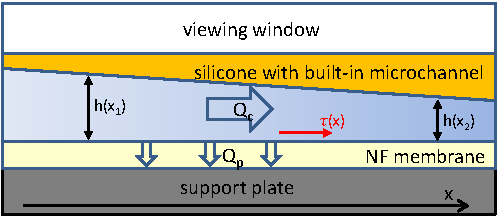
\includegraphics[width=0.6\textwidth]{figures/introduction/figure1_3}%
\caption{Concept schematic design of the microfluidic platform.}%
\label{figure1_3}%
\end{figure}

\begin{enumerate}
	\item Novel processing techniques development for silicone microchannel design and fabrication.
	\item Present a design of a novel modular reusable and resealable microfluidic platform which fulfills the following requirements:
	\begin{enumerate}
	\item Housing design which contains connection interfaces for injecting and discharging fluids;
	\item Flexible designed microchannels integrated in the platform;
	\item Optical transparent viewing window which allows direct investigation of the flow in the microchannel.
    \end{enumerate}
	\item Operative at high pressure (up to 10bar).
	\item Design and fabrication of the pressure and leakage test setup, pressure and leakage test of the setup.
\end{enumerate}

In the first aim we decided to develop a novel processing technique for fabricating microchannels in silicone membranes. This new rapid prototyping process should be flexible and avoid any cleanroom processes in order to save the lead times and cost. This new process should also provide proper processing precision.\\

In the second aim the preliminary microfluidic platform is designed to integrate the microchannel and the nanofiltration membranes. This part is critical because the design needs to be mechanically stable to meet the high pressure testing environment and no leakage is allowed to present at the macro-to-micro connection interfaces.\\

Then the housing of the microfluidic platform and all part which will be integrated into it are fabricated. A test setup is also designed and fabricated to pump test fluid into the platform. Pressure and leakage tests are conducted and must provide experimental results which indicate that the designed microfluidic platform is able to operate under high pressures and new improvements of the design are made according to the test results.

\subsection{Structure of This Work}
\label{1_2_2}
This master thesis is presented in five chapters. In \autoref{2} a short review on the microfluidic platforms for lab-on-a-chip applications is illustrated. Since the design in this master thesis is for high pressure applications, some state-of-the-art technologies about sealing and packaging for such applications are also explained.\\

In \autoref{3} the design and fabrication steps for every part in the preliminary design are introduced. Some details about nanofiltration membranes are presented at first. Then, the reasons for the choosing of silicone as the microchannel layer are explained by presenting two main advantages regarding the material properties and the corresponding processing technology. The fabrication of the silicone membrane and the microchannel processing technique are presented in details since this processing technique in not standard process. Finally, the housing design of the microfluidic platform is shown and the design of the pressure and leakage test setup is explained.

\begin{figure}[h]%
\centering
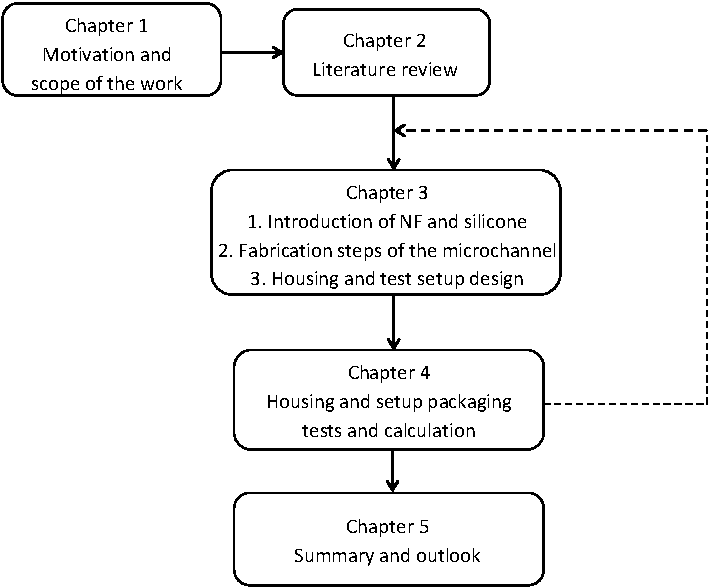
\includegraphics[width=0.8\textwidth]{figures/introduction/figure1_4}%
\caption{Work flow for reaching goals of the master thesis. The dash line shows the iterative steps to improve the performance of the design depending on the former test results.}%
\label{figure1_4}%
\end{figure}

\autoref{4} provides the packaging of both the chip housing and the test setup. In this chapter, the results of the pressure and leakage test with different housing design are presented and compared. The throughput of the flow and the filtration efficiency based on the last housing design is also calculated. In the last chapter the test results are discussed and the achievements in this thesis work are summarized. Finally, a brief overview over the further possibilities to improve the microfluidic platform design and the test setup is presented.
\chapter{Literature Review}
\label{2}
\section{Microfluidic Platforms for Lab-on-a-chip Applications}
\label{2_1}
Microfluidic platforms are defined with inner dimensions up to some hundreds of micrometers, and the microstructures inside microfluidic platforms have high surface-to-volume ratio. This provides more contact area to the channel walls for the fluid in the microchannels and this is helpful for the analysis of the near-wall micro-processes such as bacteria adhesion to surfaces. Furthermore, due to the decrease of physical dimensions microfluidic platforms also consume less fluid volumes and provide faster analysis and response times, which leads to lower cost and higher efficiency. Therefore microfluidic platforms are widely used for lab-on-a-chip applications in the field of biology procedures such as DNA analysis \cite{burns1998integrated}. Especially an emerging application area is integrating biochips into a microfluidic platform for clinical pathology like immediate point-of-care diagnosis of diseases.

\begin{figure}[ht]%
\centering
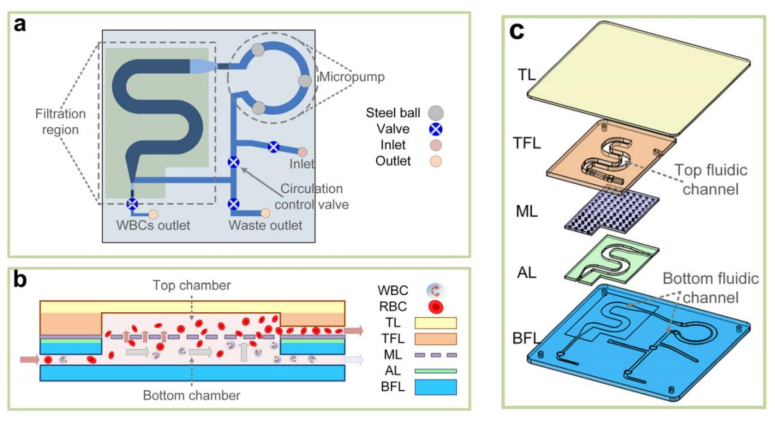
\includegraphics[width=0.8\textwidth]{figures/literaturereview/figure2_1}%
\caption{(a) Schematic of the microfiltration chip. (b) Cross-section of the chip in the filtration region. (c) Explosive view of the multilayer structure of the chip, starting from the bottom: bottom fluidic channel layer (BFL), adhesive layer (AL), Polycarbonate micro-porous membrane layer (ML), top fluidic channel layer (TFL), and top PDMS membrane layer (TL) \cite{cheng2016high}.}%
\label{figure2_1}%
\end{figure}

Cheng et al. \cite{cheng2016high} in 2015 have presented a high-throughput and clogging-free microfluidic filtration platform for on-chip cell separation from undiluted whole blood. This microfluidic platform was designed specifically for rapid separation of white blood cells (WBC) from whole blood sample for point-of-care blood pretreatment and diagnosis applications. Based on polycarbonate micro-porous membrane the white blood cells are separated with cross-flow filtration by driving the sample blood flow over the micro-porous membrane back and forth. \autoref{figure2_1} shows the schematic design of the microfiltration chip and its explosive view. This chip is composed of a micropump, which serves as the driving force of the flow, filtration region where the micro-porous membrane lays, product and waste harvesting interfaces and four valves which are used to change flow direction.

\begin{figure}[ht]%
\centering
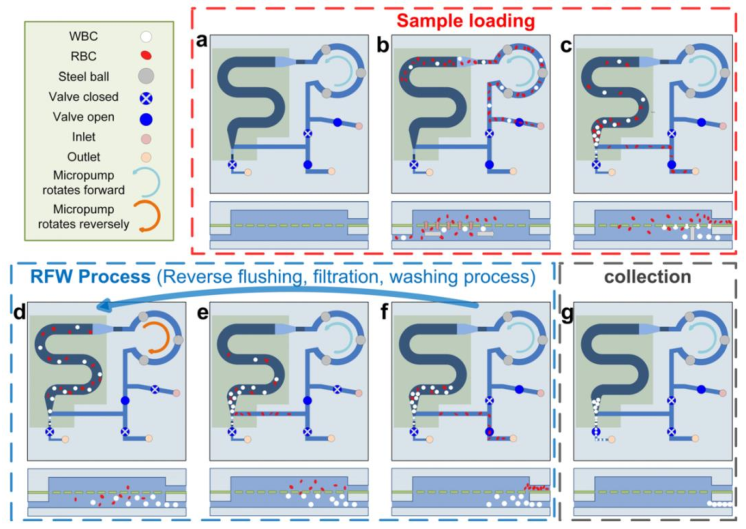
\includegraphics[width=0.9\textwidth]{figures/literaturereview/figure2_2}%
\caption{Working procedures for cell separation. (a) Load buffer. (b) Load whole blood. (c) Load buffer. (d) Reverse flushing. (e) Circulating filtration. (f) Washing away remaining red blood cells and platelets. (g) Collect white blood cell sample \cite{cheng2016high}.}%
\label{figure2_2}%
\end{figure}

The cell separation starts with sample loading, in which a volume of buffer is loaded via the inlet to rinse the chip (\autoref{figure2_2} (a)), followed by a volume of whole blood sample (\autoref{figure2_2} (b)) and then another volume of buffer (\autoref{figure2_2} (c)). Then the fluid is driven by the micropump to flow forward (counterclockwise), during which the whole blood is transported to the filtration region, where white blood cells are stopped by the micro-porous membrane and red blood cells and platelets pass through the membrane and they are harvested at the corresponding outlet. The valves are then adjusted and the micropump changes working direction to drive the fluid to flow backward (clockwise) to repeat the filtration process. This back and forth filtration process will continue working until the filtration is satisfactory. The buffer fluid acts as cleaning flow to flush away the cells trapped in micro-pores in the membrane in order to avoid blocking of the membrane.\\

Another microfluidic platform example presented by Metz et al. \cite{metz2003polyimide} is integrated with nanofiltration membranes for the application of selective delivery or probing of fluids to biological tissue (\autoref{figure2_3}). Based on cross-flow filtration specified particles in the solution can be filtered under pressure generated by a syringe pump. In the former example shown in \autoref{figure2_1} the filtration area is increased by designing the snake-shaped channel. Likewise, Metz designed microchannel structures to intensify the filtration process by increasing the contact area with meander channel geometry. 

\begin{figure}[ht]%
\centering
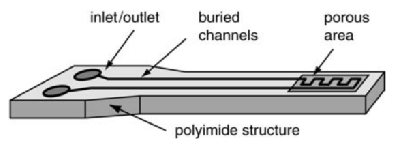
\includegraphics[width=0.5\textwidth]{figures/literaturereview/figure2_3}%
\caption{Schematic of the microchannel design for the nanofiltration process \cite{metz2003polyimide}.}%
\label{figure2_3}%
\end{figure}

\section{Laser Cutting Technology and Silicone Processing Technique}
\label{2_2}
\subsection{Laser Cutting Technology}
\label{2_2_1}

\begin{figure}[!b]%
\centering
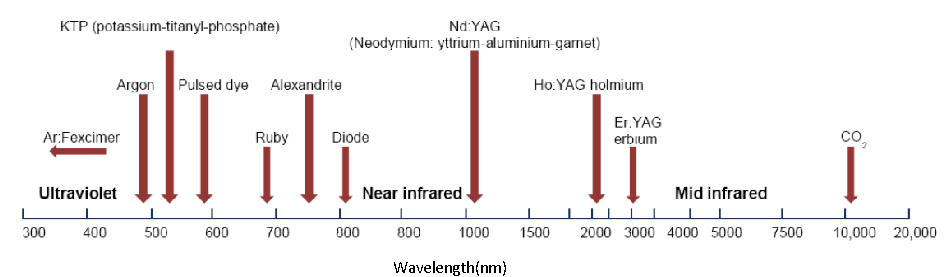
\includegraphics[width=1\textwidth]{figures/literaturereview/figure2_4}%
\caption{Classification of lasers according to the laser wavelength \cite{simpson2012basic}.}%
\label{figure2_4}%
\end{figure}

Laser cutting is now a widely used processing technique and it is more and more competitive over the conventional mechanical processing techniques. Since microstructure construction is always necessary for microfluidic applications, laser cutting has shown its ability in processing structures within the micrometer range and thus became a popular method in MEMS labs. Besides, the high processing efficiency and its processing accuracy are also satisfactory. Based on wavelength lasers can be classified into different types as shown in \autoref{figure2_4}. 

The processing mechanisms of the lasers are not always the same, depending on the laser wavelength. The mechanism of deep ultraviolet (DUV) laser ablation is a photochemical process in which the chemical bonds in the material are broken and fragments thus formed are ejected in plasma plume \cite{lasermicromachining}. Different from that, the infrared or visible lasers such as CO$_2$, Nd:YAG lasers produce fast-heating and melting of the material directly. Specifically when metal foils are processed by these lasers, the laser radiation is absorbed by the work piece within a thin surface layer, which causes a stimulation of bonded electrons and a heating of the free electrons by inverse bremsstrahlung.  Thereby the absorbed energy is deposited into the electron system and is subsequently transferred into the lattice by electron-phonon coupling, leading to the breakup of the atomic and molecular bonds and the expansion of the material (causing melting and evaporation) \cite{ref_4}. 

\begin{figure}[!b]%
\centering
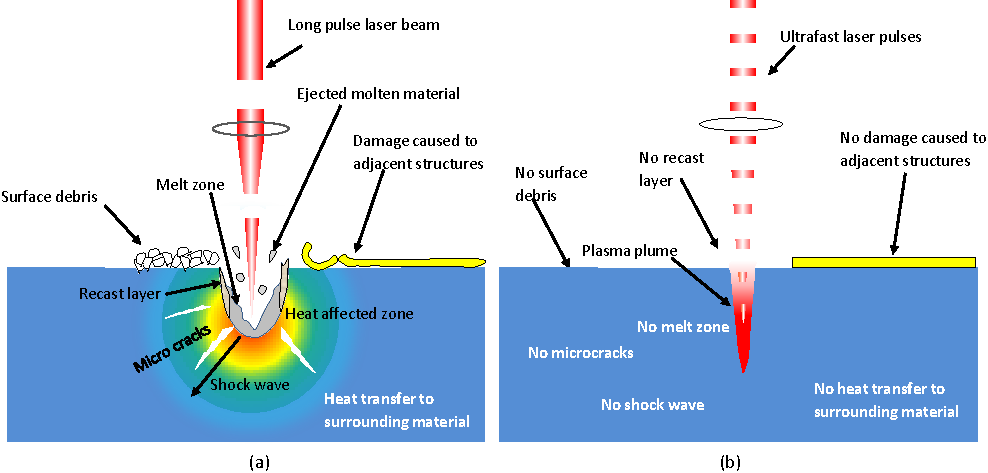
\includegraphics[width=1\textwidth]{figures/literaturereview/figure2_5}%
\caption{Comparison of processing mechanism of long pulse lasers and ultrafast pulse lasers.\cite{ref_4}}%
\label{figure2_5}%
\end{figure}

For the laser ablation process, the pulse length is an essential parameter and lasers can also be classified according to their pulse duration: long pulse lasers (pulse duration longer than 10 picoseconds) and ultrafast pulse lasers (pulse duration less than 10 picoseconds). In the long pulse regime, heat diffusion, melting and material expansion during the laser pulse are considerable. Since the laser pulse duration is longer than the heat diffusion time, the heat generated by the laser radiation will diffuse away to the surrounding area, leading to collateral damage to the surrounding area as shown in \autoref{figure2_5} (a) \cite{ref_4}. This heat diffusion also reduces the efficiency of the micromachining progress since it takes energy away from the work spot -- energy that would otherwise go into removing the material in the work piece. Besides, the absorption of long laser pulse leads to melting and evaporation of the material which can contaminate the surrounding area, produce micro-cracks and remove material over dimensions which are desired. Unlike the long pulse machining, within a ultrafast laser pulse the heat deposited by the laser into the material does not have time to move away from the work spot during the time the laser pulse is illuminating the material (\autoref{figure2_5} (b)) \cite{ref_4}. Therefore the energy is fully absorbed by the material and thus the material is converted from a solid state directly to a gas phase without first going through a melt phase, taking away almost all the heat with it. Consequently, very little heat is left behind to damage the material, thus providing much better processing accuracy than the long pulse lasers \cite{chichkov1996femtosecond}.

\subsection{Silicone Processing Technique}
\label{2_2_2}
Silicones are known as polymers that include any inert, synthetic compound made up of repeating units of slogans, which is a chain of alternating silicon atoms and oxygen atoms, frequently combined with carbon and/or hydrogen \cite{moretto2000silicones}. PDMS, widely used in cleanrooms for the process of soft lithography, is a well-known silicone. Silicones exhibit many useful characteristics including low thermal conductivity, low chemical reactivity, low toxicity, thermal stability, electrical insulation properties. These characteristics make silicones useful in many products, especially for medical applications due to its low chemical reactivity and low toxicity. Many of elements in the microfluidic devices are also made of slickness, leading to many kinds of silicone processing technologies.\\

\begin{figure}[h]%
\centering
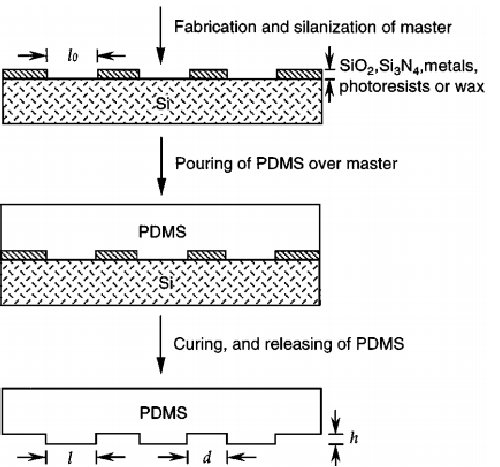
\includegraphics[width=0.6\textwidth]{figures/literaturereview/figure2_6}%
\caption{Fabrication of the PDMS stamp or mold \cite{xia1998soft}.}%
\label{figure2_6}%
\end{figure}

The mainstream microfabrication technology for patterning silicones is soft lithography. Xia et al. presented their soft lithography technology for patterning different geometries of microstructures \cite{xia1998soft}. The key element of soft lithography is an elastomeric block with patterned relief structures on its surface and this element acts as the stamp or mold for the mass fabrication of silicone microstructures. \autoref{figure2_6} shows the procedure for fabricating PDMS stamps from a master having relief structures on its surface. The master is rigid and fabricated using microlithographic techniques such as photolithography or e-beam writing.  After the fabrication and silanization of the master, liquid PDMS is poured over the master and makes conformal contact with the surfaces, forming a patterned PDMS stamp or mold after curing. 

\begin{figure}[h]%
\centering
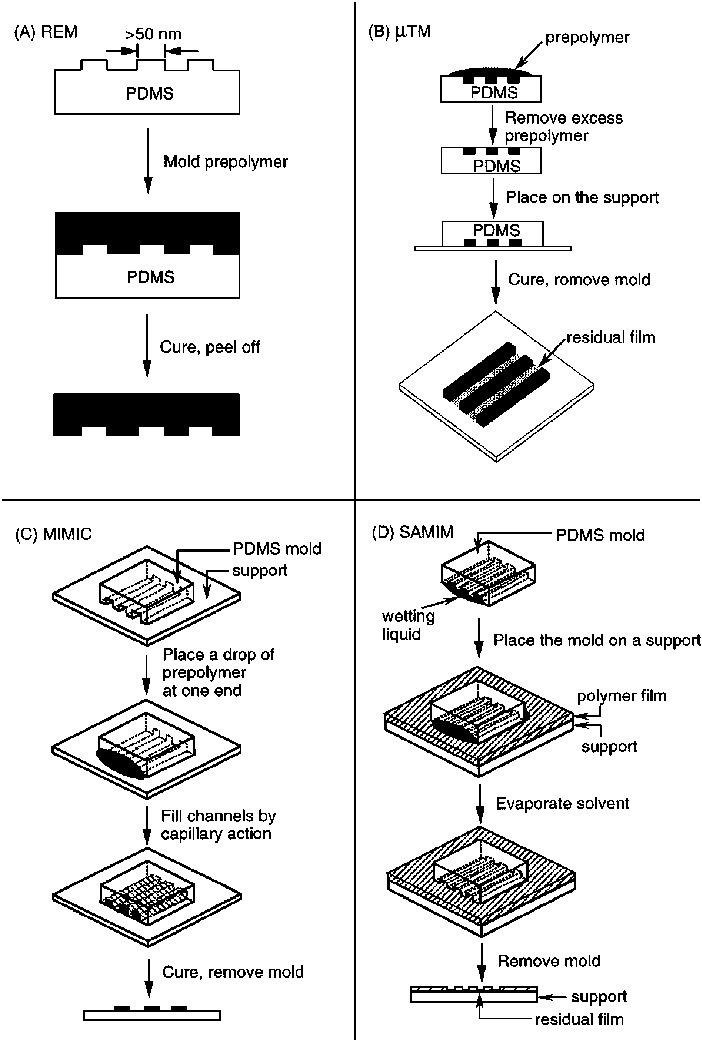
\includegraphics[width=0.65\textwidth]{figures/literaturereview/figure2_7}%
\caption{Schematic illustrations of procedures for (a) Replica Molding (REM), (b) Microtransfer Molding ($\mu$TM), (c) Micromolding in Capillaries (MIMIC), and (d) Solvent-assisted Micromolding (SAMIM) \cite{xia1998soft}.}%
\label{figure2_7}%
\end{figure}

Based on this silicone mold several techniques have been developed by Xia for the mass-producing of microstructures. \autoref{figure2_7} (a) shows the procedure of Replica Molding (REM) technique. The liquid silicone is casted to the PDMS mold and is peeled off after curing. The structures in this silicone are complementary to those on the PDMS mold and are the same to those on the original master. \autoref{figure2_7} (b) shows the procedure of Microtransfer Molding ($\mu$TM) technique. A thin layer of liquid prepolymer is applied to the patterned surface of a PDMS mold and the excess liquid is removed. This mold, filled with the prepolymer, is then placed in contact with the surface of a substrate. The prepolymer is then cured to solid and forms the microstructure on the surface of the substrate when the mold is peeled away. \autoref{figure2_7} (c) presents the Micromolding in Capillaries (MIMIC) technique. In MIMIC a PDMS mold is placed on the surface of a substrate to form empty channels between them and a low-viscosity prepolymer is then placed at the open ends of the channels. This liquid then fills the channels by capillary action and after curing the patterned microstructures are revealed by removing the PDMS mold. In \autoref{figure2_7} (d) the Solvent-Assisted Micromolding (SAMIM) technique is presented. SAMIM generates relief structures in the surface of a material using a good solvent that can dissolve the material without harming the PDMS mold. The PDMS mold is wetted first with the solvent and brought into contact with the surface of the substrate. The solvent then dissolves a thin layer of the substrate. The patterned relief structure complementary to that in the surface of the mold is then formed when the solvent dissipates and evaporates.

\begin{figure}[h]%
\centering
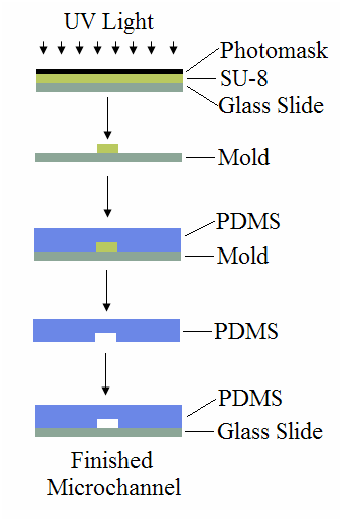
\includegraphics[width=0.4\textwidth]{figures/literaturereview/figure2_8}%
\caption{Schematic for microchannel fabrication procedure \cite{boyajian2010microchannel}.}%
\label{figure2_8}%
\end{figure}

Likewise, Boyajian has presented a similar technique specifically for microchannel \cite{boyajian2010microchannel}. \autoref{figure2_8} shows the schematic procedure for the microchannel fabrication. The master mold is fabricated also by soft lithography technique. The SU-8 photoresist is spin-coated on top of a glass slide and then is covered by photomask. The photoresist is then patterned by UV light exposure and liquid PDMS silicone is poured on top of the mold to the desired thickness. After curing, the PDMS is peeled off of the mold and is bonded to a new glass slide and the microchannel is formed.

\section{Sealing and Packaging of High Pressure Microfluidic Systems}
\label{2_3}
To ensure the reusability and resealability for high pressure microfluidic applications, the sealing and packaging technology of the device is still a significant technical challenge. There are several sealing and packaging processes that can be summarized into two main categories: permanent sealing and nonpermanent sealing. Permanent sealing can be realized by a lot of different bonding and gluing processes and is widely used in microfluidic devices. Nonpermanent sealing is realized by applying O-rings or only by conformal contact. For the application in this thesis work, nonpermanent sealing technique is required since the microfluidic platform should be resealable and reusable for the integration of many different membrane samples.\\

\begin{figure}[!b]%
\centering
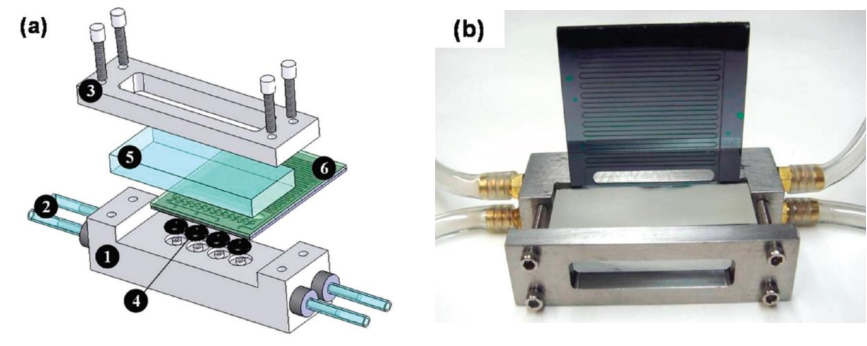
\includegraphics[width=0.8\textwidth]{figures/literaturereview/figure2_9}%
\caption{(a) Scheme of a high pressure microfluidic assembly: (1) compression part, (bottom) with modular fluidics inlet/outlet ports, (2) cooling fluid pathway, (3) compression part (top), (4) O-rings and grooves, (5) Pyrex plate for optical access, (6) microreactor. (b) Image of the final assembly \cite{marre2010design}.}%
\label{figure2_9}%
\end{figure}

Marre et al. \cite{marre2010design} in 2010 has presented a sealing method for high pressure and high temperature microreactors. For easy fabrication and easy interchange of microreactors, nonpermanent connections based on the compression of O-rings are applied. \autoref{figure2_9} shows the scheme of the microreactor assembly. The compression chuck consists of two stainless steel parts compressing the microreactor (part 1 and part 3 in \autoref{figure2_9} (a)). The bottom one is integrated with tubes (part 2) for the cooling of the microreactor while the upper part aims at compressing the microreactor against O-rings (part 4) and holding pressure. The upper part is equipped with a window for visualization of the microreactor. Therefore in order to ensure good homogeneity in the compression, an additional Pyrex part (part 5) is placed in between the microreactor and the upper part.

While nonpermanent sealing provides great convenience for the resealability and reusability of the microfluidic device, the pressure it can withstand is not always as high as certain permanent connection methods. Therefore adhesive assisted sealing or bonding techniques presents in most of the microfluidic devices. Li et al. \cite{li2014usb} have presented an adhesive based sealing technique for developing microfluidic chips on printed circuit boards (PCB) as shown in \autoref{figure2_10}. This microfluidic chip is fabricated on PCB in order to provide fast monitoring of the flow and a more compact integration. The geometry of the microchannel is at first designed and printed to the copper layer of PCB by standard PCB etching technology. The fabricated PCB is then covered by a glass slide, which is coated with a UV-curable adhesive. The microchannels are completed after the UV solidification of the adhesive.

\begin{figure}[ht]%
\centering
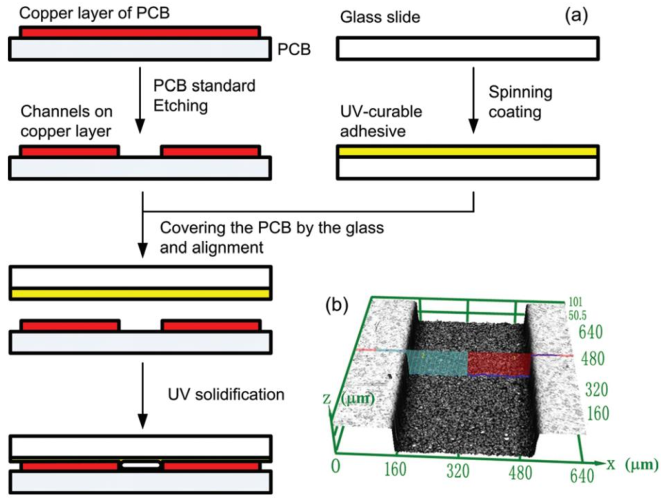
\includegraphics[width=0.7\textwidth]{figures/literaturereview/figure2_10}%
\caption{(a) Fabrication process of the microchannels on a PCB. (b) 3D topography of a fabricated microchannel on a PCB \cite{li2014usb}.}%
\label{figure2_10}%
\end{figure}













\chapter{Design and Fabrication} 
\label{3}
The idea of this microfluidic platform is to design a housing package with flexible built in microchannels. As illustrated in \autoref{1_2_1} and as is shown in \autoref{figure3_1}, the suspension is supposed to flow in a microchannel with well-defined variable depth so that the hydrodynamic environment is controllable and quantifiable. In this thesis work the microfluidic platform design, fabrication and integration are the main task and initial pressure and leakage tests are also conducted. However, the study of adhesion features of the bacteria is not included due to time limit.

\begin{figure}[ht]%
\centering
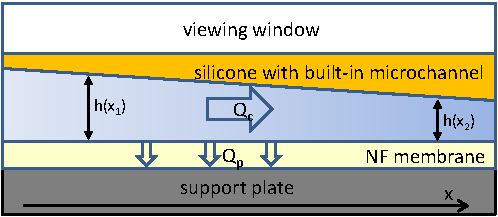
\includegraphics[width=0.6\textwidth]{figures/designandfabrication/figure3_1}%
\caption{Schematic design of the integrated structures in the microfluidic platform}%
\label{figure3_1}%
\end{figure}

To observe the filtration features during separation, the channels in which the suspension flows should be visible. Therefore the housing for the silicone channels and the nanofiltration membrane should be totally optically transparent. Moreover, because this microfluidic platform is designed also for high pressure applications, a stable sealing of the whole housing under high pressure is needed for the leakproofness. Apart from that, the sealing and packaging procedure must be reusable and resealable in order to provide the possibility of assembling and disassembling of the housing many times to replace the nanofiltration membranes. \\

In this chapter, the basic information of nanofiltration membranes and the advantages of using silicone membranes as a basis for sealing gaskets are explained and discussed. Also, the fabrication steps of the silicone membranes are introduced. To machine microchannels in these silicone membranes a novel laser processing technology is explained and analyzed, including machining through-cut microchannels and microchannels with variable depth. The flip-chip transferring steps of the silicone microchannel followed to attach the soft silicone membrane with built in microchannels to a glass slide as a carrier are introduced. All the fabrication steps above have been considered to be reproducible and flexible for further developments. At last, several housing designs are performed to assemble the microchannels with nanofiltration membrane to contribute the microfluidic platform and a test setup is designed for pressure and leakage tests of this platform. 

\section{Nanofiltration Membranes}
\label{3_1}
Nanofiltration refers to a special membrane process which rejects particles on the nanometer size scale. The nanofiltration membrane is a type of pressure-driven membrane with properties between those of reverse osmosis (RO) and ultrafiltration (UF) membranes. Nanofiltration membranes have applications in several areas such as water treatment for drinking water production as well as wastewater treatment. They also offer many advantages such as low operation pressure, high flux, and high retention of multivalent anion salts, relatively low investment and low operation and maintenance costs \cite{hilal2004comprehensive}. \\

In this master thesis, the microfluidic platform is built for testing the adhesion features of bacteria when permeate flow is introduced by the nanofiltration membrane. Suspensions containing colloidal particles like bacteria are supposed to be filtered by such nanofiltration membrane when flowing over and the phenomena such as deposition and adhesion as well as bacteria colony growth is to be investigated during and after the filtration. The type of the nanofiltration membrane selected for this test is NF90.

\section{Silicone Microchannels}
\label{3_2}
The microchannels are built in 200~$\mathrm{\mu m}$ thick silicone membranes with an inlet and an outlet reservoir and a 1mm wide microchannel connecting the inlet and the outlet. Because silicone is soft material, this silicone membrane is then glued to a microscope glass slide which acts as the mechanical microchannel carrier.

\subsection{Advantages of Silicone Material }
\label{3_2_1}
In this master work, the type of silicone selected is WACKER Silicone M 4641 A/B. It is composed of two components: silicone compound and platinum catalyst which are mixed with a mass ratio 10:1. The basic technical data is listed in \autoref{table3_1}.\\

\begin{table}[!h]
    \centering
    \caption{Product data of WACKER silicone M 4641 A/B \cite{wackersilicone}}
    \begin{tabular}{ll}
    \toprule
    Typical general characteristics	& Value \\
    \midrule
    Viscosity at ${23}^{\circ}$C & 30000 mPa s \\
    Color & Translucent \\
    Hardness Shore A & 43 \\
    Elongation at break & > 300\% \\
    \bottomrule
    \end{tabular}
    \label{table3_1}
\end{table}

To obtain direct observation of microscopic processes that occur at the nanofiltration membrane surface the transparency of the microchannel is needed. Therefore the microchannel should be built in a material which has good optical transparency and hence this silicone material is applicable here. Apart from that, silicone is non-toxic and does not release any particles; hence the solutions would not get contaminated. Another reason of choosing silicone is its good sealing performance. Silicone can adhere to glass well without additional adhesive by conformal contact and that is also the reason why glass slide is chosen as the microchannel carrier. Silicone also seals well to other material since it can deform to provide leak-free sealing. Last but not the least, stock silicone membranes of a fixed thickness can be cast in a mold. Sections of this stock membrane can then be cut, adhered to a glass slide and laser patterned for multiple chips. \\

\subsection{Advantages of Laser Rapid Prototyping}
\label{3_2_2}
There are already methods to pattern microchannels in silicone materials. One of them is the soft lithography as illustrated in \autoref{2_2_2}. This method relies on the fabrication of the mold, to which the silicone is casted. The fabrication technology for fabricating the mold is photo lithography, which is cleanroom process and needs multiple complex procedures such as mask deposition and patterning. However, any cleanroom processes in this thesis work are supposed to be avoided since they are complicated and time-consuming. Besides, different casting molds are needed for different microchannel designs, leading to low design flexibility and high cost. Therefore, to save time and cost, laser rapid prototyping (LRP) processes are taken into account.\\

A laser is a device that emits light through a process of optical amplification based on the stimulated emission of electromagnetic radiation \cite{ref_4}. Laser cutting is done by focusing a beam of high intensity energy on the material to be cut, which causes it to either melt or evaporate, depending mostly on the laser intensity and the laser pulse width. Laser cutting machines can be classified into two main categories according to the laser wavelength: deep ultraviolet (DUV) (about 200-300nm) lasers and infrared or visible lasers such as CO$_2$ and Nd:YAG lasers (0.5-10$\mu$m). The ablation mechanism of the former lasers is a photochemical process in which the chemical bonds in the material are broken while that of the latter lasers are to heat and melt the material directly \cite{lasermicromachining}. The laser which is available in our lab is a Nd:YAG laser (DPL Smart Marker II from ACI company) . The wavelength of this laser is 1064nm and the pulse length can be adjusted within the range 15-100ns. The pulse repetition rate can also be user-defined from 1 to 100kHz. The basic mechanism of laser cutting of this laser is shown in \autoref{figure3_2} and can be summarized as follows:

\begin{itemize}
	\item A high intensity beam of infrared light is generated by the laser.
	\item This beam is focused onto the surface of the work piece by means of lens.
	\item The focused beam heats the work piece and establishes a very localized melt.
	\item This localized area of work piece is removed thus generating a cut.
\end{itemize}

\begin{figure}[ht]%
\centering
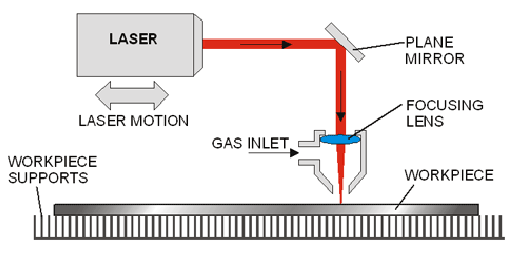
\includegraphics[width=0.6\textwidth]{figures/designandfabrication/figure3_2}%
\caption{Schematic of laser cutting \cite{lasercut}.}%
\label{figure3_2}%
\end{figure}

The machining accuracy of the laser is enough for the work in this thesis. One prominent advantage of LRP is the flexibility. The microchannel models are firstly constructed by computer-aided design and they could be directly subjected to the implementation of LRP. This means the geometric design of the microchannel could be quite flexible and fast. To conclude, the main advantages of LRP can be summarized as follows:

\begin{itemize}
	\item Processing procedures are simplified and fast.
	\item Cost of the processing is low.
	\item Machining precision is acceptable.
	\item Microchannel design is fast and flexible.
\end{itemize}

\section{Silicone Casting}
\label{3_3}
The type of silicone used here is WACKER silicone M 4641 A/B. It is a two-component silicone rubber which vulcanizes at room temperature as mentioned in \autoref{3_2_1}. Component A is the platinum catalyst while component B is the silicone and the mix ratio of the two components is 1:10 (mass). \\

First of all, all the tools and the containers which will be used should be cleaned by acetone and isopropanol. Therefore most of the dusts are removed so that the silicone will not be contaminated.
Then the silicone components A and B are measured with 1:10 weight ratio in a container. A weighing scale is used for the weight measurement. The compounds should be stirred for a few minutes with a spatula until it is thoroughly mixed.\\

The mixture is then placed in a vacuum chamber for degassing since a lot of air is introduced during the stirring. The degassing process lasts for 15 minutes so that the most of the air can be removed from the silicone mixture.\\

After the degassing process the silicone mixture is poured to the casting mold uniformly shown in \autoref{figure3_3}. Then a metal lid is compressed against the silicone by screws and the silicone will fill in all the gaps in the mold. The depth of the casting area is 200$\mu$m and that is the thickness of the cured silicone membrane. After 12 hours (cure time) the mold could be opened and the silicone membrane could be peeled off.\\

\begin{figure}[!t]%
\centering
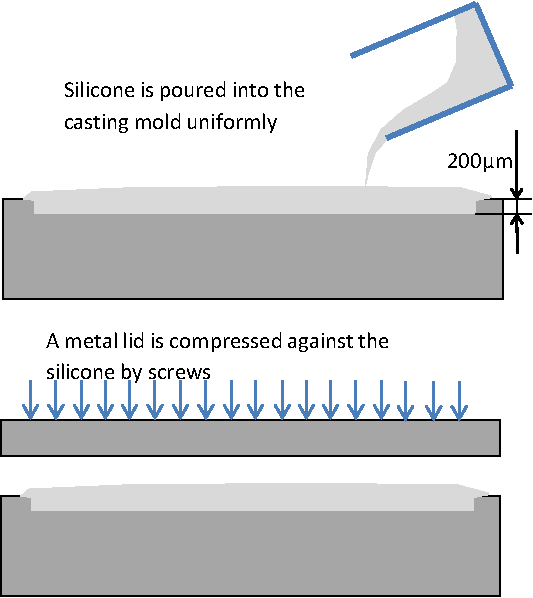
\includegraphics[width=0.6\textwidth]{figures/designandfabrication/figure3_3}%
\caption{Silicone casting steps}%
\label{figure3_3}%
\end{figure}

\section{Design and Fabrication of Silicone Microchannels}
\label{3_4}
The 200$\mu$m thick silicone membranes produced from the former step are at first cut to the size of a glass slide (76 $\times$ 26mm) and attached to the glass slide. The glass slide acts as the mechanical carrier of the membrane because the silicone is too soft. This silicone membrane with glass slide is to be patterned by the laser. \\

The silicone membrane is transparent to the laser so that it does not absorb any laser beam. Therefore it cannot be cut directly. To solve this problem the other side of the silicone is attached to a steel sheet (from H+S Pr\"azisions Folien, CrNi-Stahl, hardness: 1.4310, thickness: 110$\mu$m) which will be ablated first. In this thesis work, this steel sheet is applied to all laser patterning of silicone membrane. Due to the material properties, changing this metal material may result in a change of the laser parameters. \\

When ablated, the metal melts or even evaporates and will release high temperature ablated particles. These particles with certain kinetic energy will diffuse and some of them move towards the silicone membrane and burn the silicone membrane at the same time and thus the silicone membrane is patterned by this indirect laser ablation. The heat energy and the kinetic energy both play a role in the ablation of silicone membrane and define the depth and the quality of the ablation. The main advantage of this indirect ablation is minimized thermal damage to the silicone membrane. Because the laser under use generates long-pulse laser waves, it will heat the adjacent work piece as well rather than just ablate the area where the laser spot focalizes as illustrated in \autoref{2_2_1}. Since steel is a far better thermal conductor than the silicone, the heat in the locally generated hot spot during ablation is quickly transported away, thus the thermal damage to the silicone membrane is reduced. The laser processing flow is shown as \autoref{figure3_4}:\\

\begin{figure}[ht]%
\centering
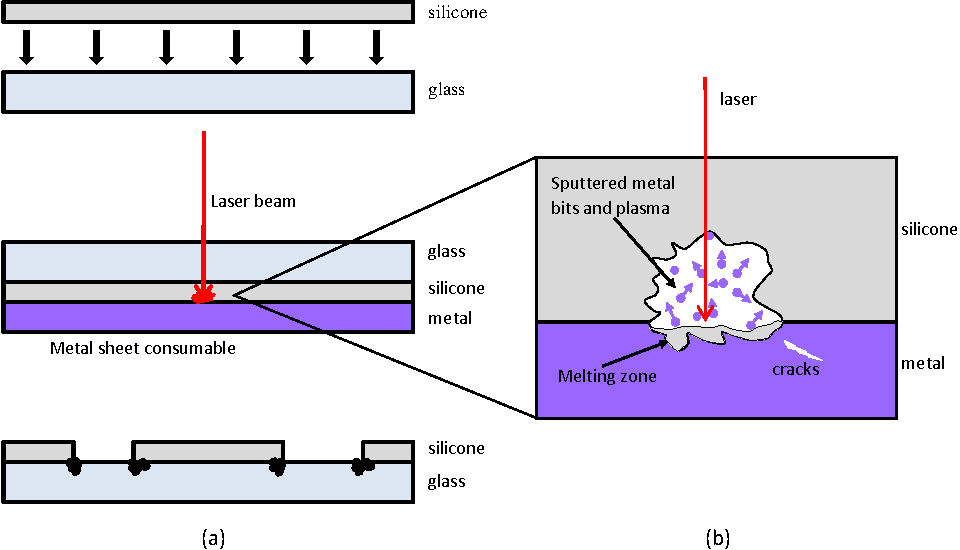
\includegraphics[width=0.8\textwidth]{figures/designandfabrication/figure3_4}%
\caption{(a) Process flow of the silicone machining process, (b) Detail view of the laser working.}%
\label{figure3_4}%
\end{figure}

A jig is designed for the silicone laser processing to hold the glass, silicone and metal layers. The glass with the silicone membrane is compressed to the metal sheet to ensure full contact. This compression is realized by uniformly distributed screws. \autoref{figure3_5} shows the geometry design of the jig.\\

\begin{figure}[t]%
\centering
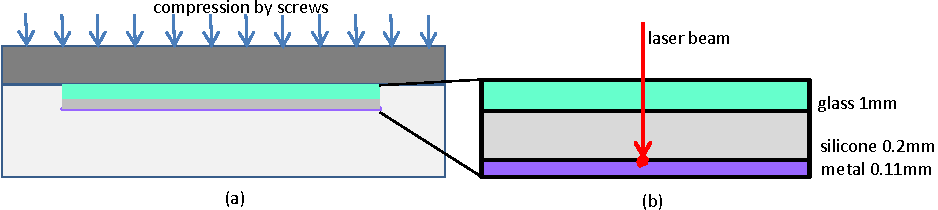
\includegraphics[width=0.8\textwidth]{figures/designandfabrication/figure3_5}%
\caption{(a) Design of the jig, (b) Thickness of each layer.}%
\label{figure3_5}%
\end{figure}

There are 5 main parameters to be set for the laser: power, frequency, speed of cutting, pulse width and number of passes. The parameter power is the power of the laser source presented with percentage to its maximum power and the speed of cutting is the moving speed of the laser beam along the processing path at the surface of the work piece as shown in \autoref{figure3_6} (a). \autoref{figure3_6} (b) illustrates the definition of frequency and pulse width. The laser pulse is a square wave and the pulse repetition rate is the parameter frequency, which is the reciprocal of the pulse period. The pulse width is the time duration in which laser beam presents. The duty ratio of the laser beam as well as the pulse period defines the average laser power with certain laser power input. In other words, longer pulse width and/or shorter pulse period (higher frequency) will result in higher average laser power.\\

\begin{figure}[b]%
\centering
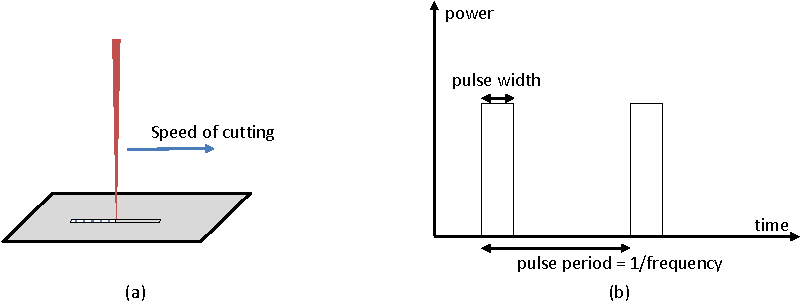
\includegraphics[width=0.9\textwidth]{figures/designandfabrication/figure3_6}%
\caption{(a) The speed of cutting is the moving speed of the laser beam along the processing path. (b) Definition of pulse width and frequency.}%
\label{figure3_6}%
\end{figure}

Each of these parameters can affect the machining quality much and these parameters interact with each other as well. To gain the optimal parameter set, the laser parameter test should be conducted at first. The laser parameter test is described as follows:\\

\begin{itemize}
	\item Two parameters are chosen as the variable for test. Here power and frequency are used as an example. Keep all the other parameters fixed.
	\item Set the range of the power and frequency.
	\item Characterize the processing quality under the microscope after machining. Choose the square with the best processing quality and record the corresponding power and frequency as shown in \autoref{figure3_7}.
	\item Switch the variable to other parameters while setting the power and frequency fixed to the former optimal value. Repeat the former steps to find all the optimal parameters which forms the optimal parameter set.
\end{itemize}

\begin{figure}[h]%
\centering
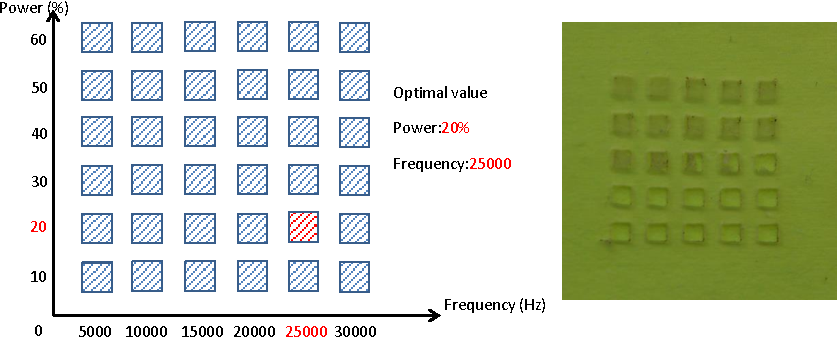
\includegraphics[width=0.9\textwidth]{figures/designandfabrication/figure3_7}%
\caption{Laser parameter test, assume the processing quality of the highlighted square is the best, the best power and frequency value is determined. Left side: schematic. Right side: test picture.}%
\label{figure3_7}%
\end{figure}

\subsection{Through-cut Microchannels}
\label{3_4_1}
The first stage of the work is to machine through-cut microchannels with surrounding additional sealing gaskets to verify the feasibility of indirect ablation and its processing quality as well. There are two possibilities to process the through-cut microchannels as shown in \autoref{figure3_8}.\\

\begin{figure}[h]%
\centering
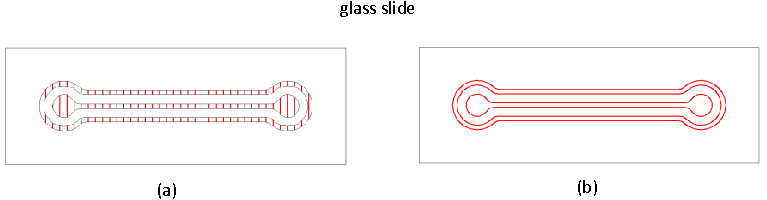
\includegraphics[width=0.9\textwidth]{figures/designandfabrication/figure3_8}%
\caption{Two methods to process through-cut microchannels. (a) Full area (red stripes represent laser cutting path) of the channel is processed. (b) Only the contour (red lines) of the channel is processed.}%
\label{figure3_8}%
\end{figure}

The first possibility is the full area scanning of the laser beam as shown in \autoref{figure3_8} (a). The filling lines represent the cutting path of the laser beam and in this way the whole area of the microchannel is ablated. However, due to the long cutting path the processing time to cut a microchannel can be more than one hour, which is of low machining efficiency. The second possibility is to only cut the contour of the microchannel as shown in \autoref{figure3_8} (b). The silicone inside the channel will still remain intact and can be peeled off after the laser processing. In this way the length of the cutting path is dramatically reduced compared to the first method and the processing time is also reduced to only around ten minutes, providing a quite efficient laser cutting. Therefore the second strategy is applied here to machine through-cut microchannels.\\

First of all, the laser parameter set is found and listed as shown in \autoref{table3_2}:

\begin{table}[!h]
    \centering
    \caption{The optimal laser parameter set for through-cut channels}
    \begin{tabular}{ll}
    \toprule
    Parameter  &   Value \\
    \midrule
    Power  &  62$\%$ \\
    Frequency  &  6900Hz \\
    Cutting speed  &  10mm/s \\
    Pulse width  &  3$\mu$s \\
    Processing passes  &  60\\
    \bottomrule
    \end{tabular}
    \label{table3_2}
\end{table}

Several different geometries of the microchannel are designed by CAD and machined by the laser. A jig is designed for the laser process. As shown in \autoref{figure3_9}, there is front window in the jig, through which the laser beam reaches the metal sheet and only this area can be processed. The four edges of the glass slide are under compression to keep the silicone membrane fixed during laser ablation. During the processing, only the outline of the microchannel is cut. \autoref{figure3_10} shows how the processing result looks like: there is a lot of black powder around the channel right after the processing and this powder is composed of both the burned metal sheet and the burned silicone membrane. After wiping these black residues away with laboratory cotton swabs the outline on the channel could be viewed clearly. The metal sheet is seriously ablated but not through-cut so that the jig is not harmed by the laser. The silicone membrane is through-cut and the channel connects the inlet and outlet reservoir. Nevertheless, the glass slide is also harmed a bit by the laser and thus it should be replaced afterwards. This transfer process will be illustrated in \autoref{3_4_3}.

\begin{figure}[ht]%
\centering
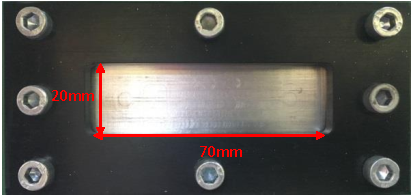
\includegraphics[width=0.5\textwidth]{figures/designandfabrication/figure3_9}%
\caption{Jig for the laser processing, the window defines the processing area.}%
\label{figure3_9}%
\end{figure}

\begin{figure}[ht]%
\centering
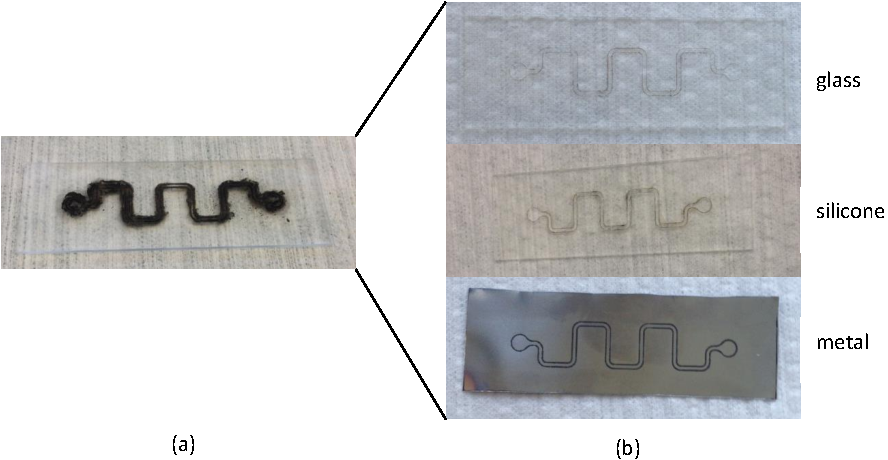
\includegraphics[width=0.95\textwidth]{figures/designandfabrication/figure3_10}%
\caption{Laser process results. (a) Before cleaning and separating the stack. (b) After cleaning and separating, silicone is through-cut, but the glass slide is also harmed by the laser.}%
\label{figure3_10}%
\end{figure}

\subsection{Flip-chip Transferring of the Silicone Microchannel}
\label{3_4_2}
For initial pressure and leakage test, through-cut microchannels with surrounding sealing gasket are needed. However, the glass slide will also get cut a bit by the laser beam as shown in \autoref{figure3_11}. As a result, this glass slide cannot be used as the mechanical carrier of the silicone membrane anymore because this cutting trace would be the weak point and even break when it is working under high pressure. Therefore the silicone membrane with microchannels built in should be transferred to a new glass slide.\\

\begin{figure}[h]%
\centering
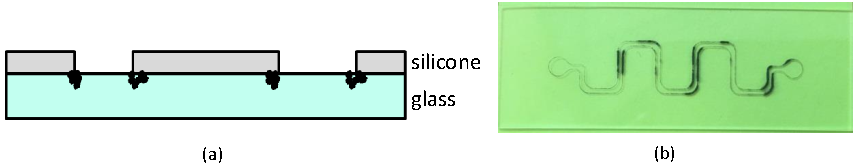
\includegraphics[width=0.9\textwidth]{figures/designandfabrication/figure3_11}%
\caption{(a) Side view of the damaged glass slide, (b) Top view of the damaged glass slide.}%
\label{figure3_11}%
\end{figure}

First of all, the front side of the silicone membrane is cleaned by ethanol. The black ablated residue should be wiped away by laboratory cotton swabs with ethanol before the transfer process. The other side of the silicone membrane which is in contact with the glass slide is also partially contaminated by the residue (black dots shown as \autoref{figure3_11} (a)) and could not be totally cleaned. It will be cleaned when the silicone is transferred to a clean slide and this surface is now exposed.\\

To glue the silicone membrane to the new glass slide the main challenge is the difficulty of obtaining a uniform thickness along the new glass slide surface, and avoiding clogging of the microfluidic channels during the curing of the adhesive. Besides, the adhesive should be optically transparent so that the view of the microchannel will not be affected by the adhesive. Since the surface energy of the silicone membrane is extremely low, only a few adhesives could thoroughly wet out the bonding interface. Besides, most adhesives such as normal adhesives (e.g. UHU Alleskleber) or epoxy based adhesives (e.g. UHU 5-Minute Epoxy) cannot glue silicone at all. Superglue (e.g. Loctite 648, Gel Sekundenkleber) is able to glue silicone, but it cures within several seconds so that there is no enough time to uniformly distribute it. And it also shrinks during curing which will cause deformation to the microchannel. At last the silicone itself is applied as the glue since it shows good compatibility to glass and to itself and will not introduce any impurities since it is the material which the silicone membrane is made from.\\

\begin{figure}[h]%
\centering
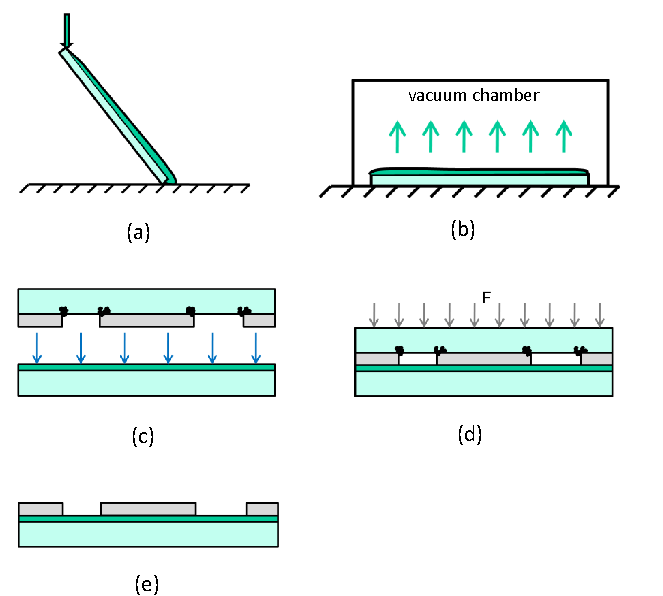
\includegraphics[width=0.8\textwidth]{figures/designandfabrication/figure3_12}%
\caption{process flow of the flip-chip transfer process of the silicone membrane.}%
\label{figure3_12}%
\end{figure}

\autoref{figure3_12} illustrates the steps transferring the silicone membrane to the new glass slide. Figure (a) shows the deposition of the glue (fluid silicone). Since the viscosity of the fluid silicone is too large for it to flow over the glass, the silicone is firstly diluted in DOW CORNING silicone solvent OS-20 \cite{os_20} to increase its fluidity. The mass mix ratio of the silicone to the solvent is 1:2. When the silicone dissolves in the solvent thoroughly by stirring, the solution is poured onto the new glass slide. To make the adhesive layer as thin as possible, which is good for a better view into the channel and does not introduce any change to the channel geometry, the glass slide is kept tilted for 1 min until most of the solution has flowed away over the glass surface and in this way a uniformly distributed thin layer of the solution is achieved. Then this glass slide is put into the vacuum chamber for degassing as shown in \autoref{figure3_12} (b). Since the OS-20 solvent is volatile, it takes only 5 min for it to evaporate. The low pressure environment in the vacuum chamber during degassing accelerates the evaporation as well. After the degassing process the patterned silicone membrane together with its original glass slide is flipped and put over the silicone covered new glass slide as shown in Figure (c). To ensure seamless contact and avoid any air bubbles, an evenly distributed compression is applied over the original glass slide by the press machine as shown in Figure (d). The pressure is kept for 2 min and then the silicone will cure within the next 12 hours. When the silicone cures, the damaged original glass slide is peeled off and the front side of the silicone membrane is cleaned. Figure (e) shows the structure of the final clean silicone membrane with intact glass slide.\\



\autoref{figure3_13} shows 4 different microchannel design sample after the flip-chip transfer process. The black residues are removed and the silicone membrane is seamlessly glued to the new glass slide without any bubbles. This process also does not change the shape of the microchannel.\\
\clearpage
\begin{figure}[h]%
\centering
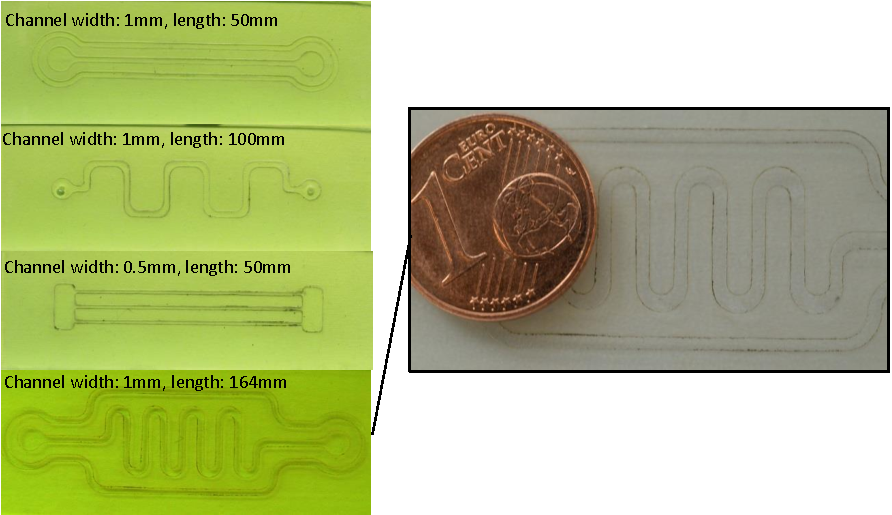
\includegraphics[width=0.9\textwidth]{figures/designandfabrication/figure3_13}%
\caption{Samples of different microchannel geometry after the flip-chip transfer process.}%
\label{figure3_13}%
\end{figure}

\subsection{Characterization of the Through-cut Microchannel}
\label{3_4_3}
After the through-cut microchannels are transferred to the clean glass slide, the processing quality is then characterized by the Laser Scanning Microscope (LSM) and the White Light Interferometer (WLI). Both results are compared for verification. Because the silicone is transparent and the reflection of the incident light from the microscope is weak, a thin layer of gold is deposited onto the silicone to enhance the reflection. \autoref{figure3_14} shows the gold coated samples.\\

\begin{figure}[h]%
\centering
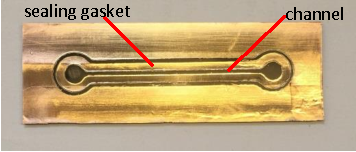
\includegraphics[width=0.5\textwidth]{figures/designandfabrication/figure3_14}%
\caption{Gold coated silicone microchannel samples, microchannel with surrounding sealing gasket.}%
\label{figure3_14}%
\end{figure}

The characterization of the microchannel is mainly the measurement of the channel depth and three-dimensional reconstruction of the microchannel. The scanning area is chosen at the channel edges, where a depth difference of 200$\mu$m should present. \autoref{figure3_15} (a) shows the channel model measured by the LSM and the depth profile across the channel. The profile gives a result of 200$\mu$m depth difference between the top surface of the silicone membrane and the channel floor, and this matches the thickness of the silicone membrane, which is 200$\mu$m. \autoref{figure3_15} (b) presents the result measured by the WLI. Likewise, the depth profile from the WLI also gives a channel depth of 200$\mu$m which matches the thickness of the silicone membrane since it is through-cut.

\begin{figure}[ht]%
\centering
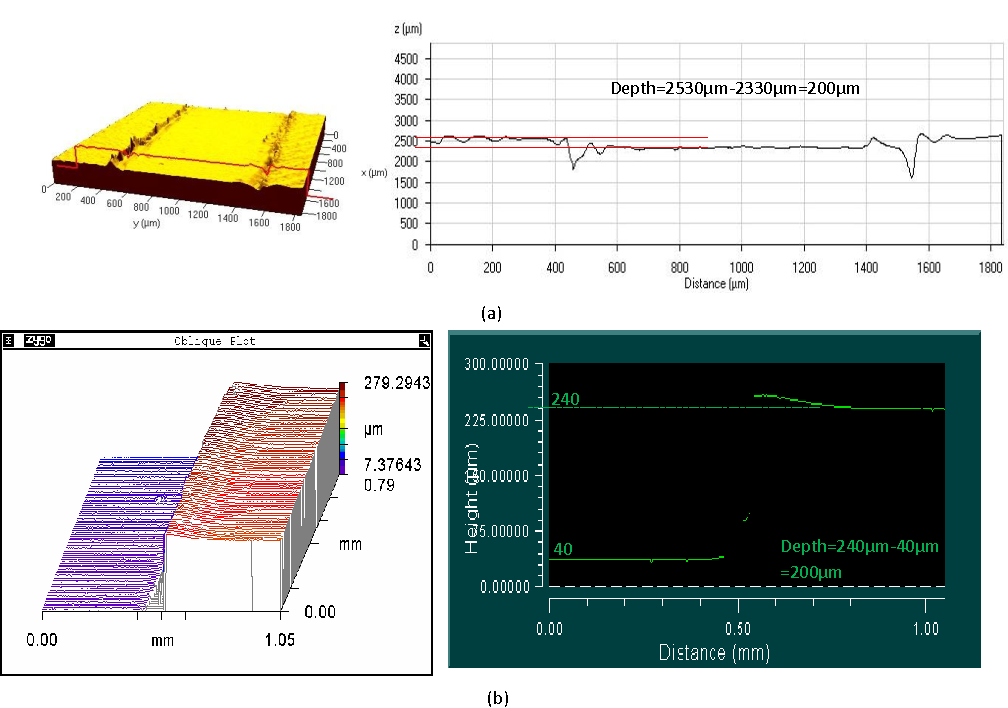
\includegraphics[width=1\textwidth]{figures/designandfabrication/figure3_15}%
\caption{(a) Result from LSM. (b) Result from WLI.}%
\label{figure3_15}%
\end{figure}

Apart from characterizing by the LSM and WLI, some directly investigated views of the channel edges are presented. \autoref{figure3_16} shows the cutting edge of straight channel. Along the edges ripples can be observed. The fluctuation of these ripples is less than 10$\mu$m, resulting in an acceptable processing accuracy.\\
\clearpage

\begin{figure}[ht]%
\centering
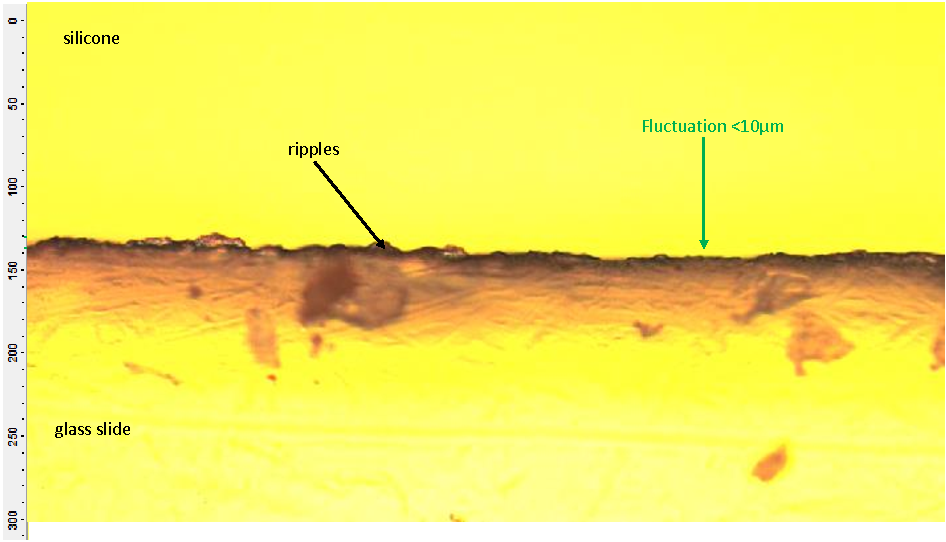
\includegraphics[width=1\textwidth]{figures/designandfabrication/figure3_16}%
\caption{Detail structure of the channel wall.}%
\label{figure3_16}%
\end{figure}

\subsection{Microchannel with Variable Depth}
\label{3_4_4}
 As illustrated in \autoref{1_2_1}, the study of bacteria adhesion features under different hydrodynamic environments are the final objective to achieve. Shear stress at the surface of the NF membrane, which may be a factor that influences bacteria adhesion, is one of these interested hydrodynamic parameters. This shear stress can be adjusted along the microchannel length by changing the depth of the microchannel. While the width of the microchannel is fixed, variation of the microchannel depth means variation of the cross-sectional area of the microchannel. Since the volumetric flow rate is fixed in a single channel test, the flow velocity will change along the length of the microchannel due to conservation of mass, leading to the variation of the shear stress on the surface of the membrane. Therefore the fabrication of microchannels with variable depth is of great interests in this master thesis work.\\

\begin{figure}[h]%
\centering
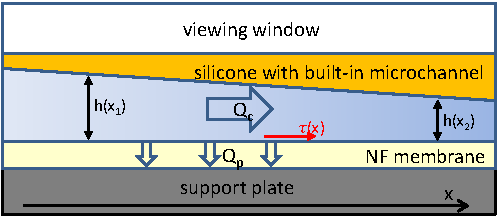
\includegraphics[width=0.6\textwidth]{figures/designandfabrication/figure3_17}%
\caption{Schematic design of integrated microchannel with variable depth.}%
\label{figure3_17}%
\end{figure}

For the through-cut channels, only the outline of the channel is cut as shown in \autoref{figure3_8}. The remaining silicone inside the channel is removed simply by the tweezers. Unlike that, all the areas in the non-through-cut channels should be processed. The channel area should be filled with stripes which are the laser cutting path rather than only processing the channel outline. \\

The laser beam is a Gaussian beam which has a waist diameter of 35$\mu$m as shown in \autoref{figure3_18} (a). This means the focused laser spot at the work piece has a diameter of 35$\mu$m. Therefore the interval of the filling lines, which are the laser scanning path, is set to 35$\mu$m as shown in \autoref{figure3_18} (b). As a result, there will not be any overlapping processing area.\\

\begin{figure}[ht]%
\centering
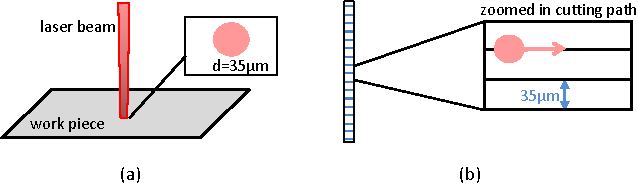
\includegraphics[width=0.8\textwidth]{figures/designandfabrication/figure3_18}%
\caption{The waist diameter of the Gaussian beam is 35$\mu$m. (b) Interval of filling lines is 35$\mu$m in order to have a smooth transition. }%
\label{figure3_18}%
\end{figure}

To find the optimal laser parameter set for a certain depth channel processing, the laser parameter tests are conducted. The test takes 6 squares as a group and only one laser parameter varies within one group. For example, when the cutting passes is under investigation, the other laser parameters are kept the same for all the 6 squares. The cutting passes increases from 20 at Square1 (S1) to 70 at Square6 (S6) as shown in \autoref{table3_3}. Therefore the cutting depth will increase from S1 to S6 and the processing quality is characterized by the microscopes.

\begin{table}[h]
    \centering
    \caption{Laser parameter set for the test}
    \begin{tabular}{ll}
    \toprule
    Other parameters & Cutting passes \\
    \midrule
    \multirow{2}{0.5\textwidth}{Speed: 10mm/s; Pulse width: 3$\mu$s; Frequency: 6900Hz; Power: 70\%} & S1: 20\ \ \ \ \ \ S2: 30\ \ \ \ \ \ S3: 40 \\
     & S4: 50\ \ \ \ \ \ S5: 60\ \ \ \ \ \ S6: 70 \\
    \bottomrule
    \end{tabular}
    \label{table3_3}
\end{table}


For the early tests, the laser power is set to a high value of 70$\%$ while the processing passes are low at 40. The other parameters are: cutting speed (10mm/s), Pulse width (3$\mu$s), Frequency (6900Hz). \autoref{figure3_19} shows the LSM picture and the WLI picture of the area which is the edge between the processed area and unprocessed area.


\begin{figure}[ht]%
\centering
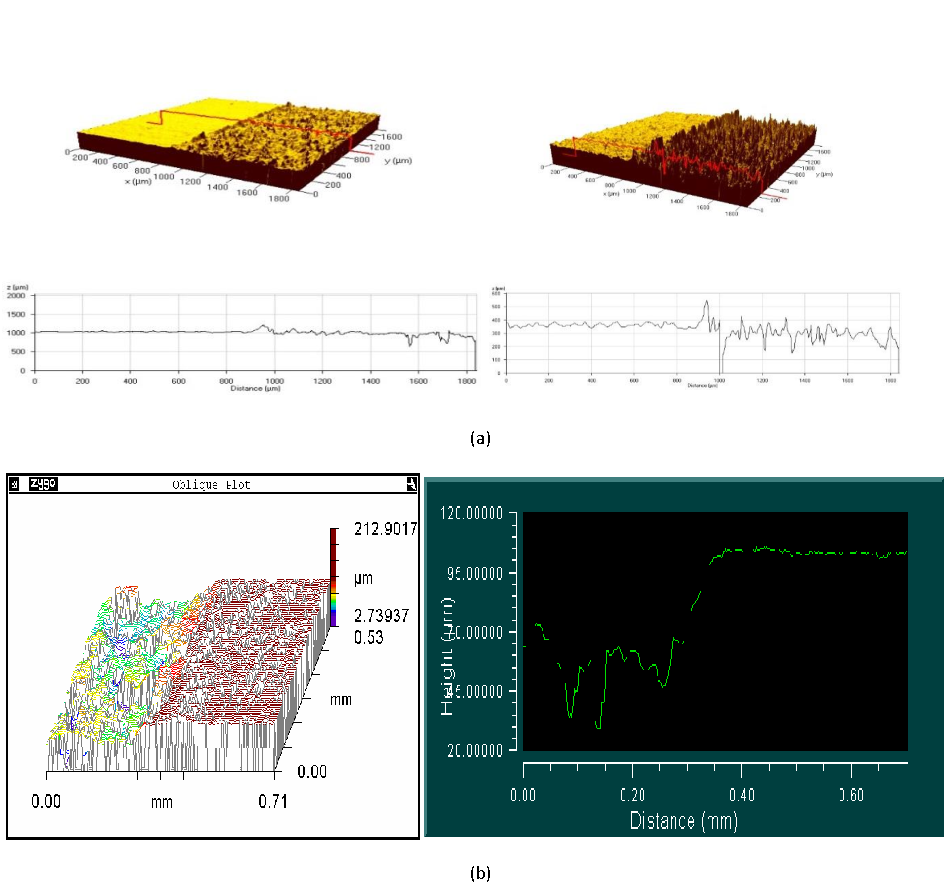
\includegraphics[width=1\textwidth]{figures/designandfabrication/figure3_19}%
\caption{(a) Processing quality picture taken by LSM. (b) Processing quality picture taken by LSM, power: 70\%, cutting speed: 10mm/s, pulse width: 3$\mu$s, frequency: 6900Hz, processing passes: 40.}%
\label{figure3_19}%
\end{figure}

From the LSM picture the cutting depth is calculated to be about 50$\mu$m, and this value matches the result measured by the WLI microscope as well. However, the surface roughness of the processed area seems to be very bad. To take a clearer view of this area and the profile in this area, this sample is also observed under the SEM as shown in \autoref{figure3_20}. The cutting depth cannot be measured by the SEM but the micro structure of the processed surface is more apparent. The silicone is ablated seriously and there are a lot of through-cut holes. Nevertheless not all the silicone is ablated which leads the processed area to be a quite porous structure. This is because the laser power is too high so that the ablated metal particles have relatively high energy which is enough to hit through the silicone membrane since the thickness of the silicone is only 200$\mu$m. Therefore the through-cut holes form. It can be predicted that if the processing passes could be increased to a proper value, all the remaining silicone will be ablated as well hence the silicone will be totally through-cut.\\

\begin{figure}[t]%
\centering
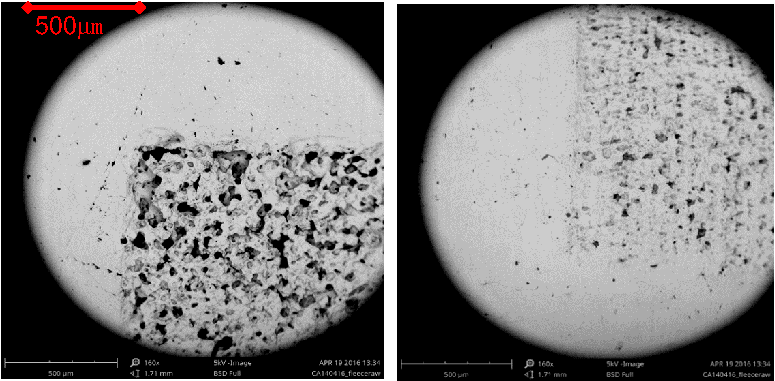
\includegraphics[width=0.9\textwidth]{figures/designandfabrication/figure3_20}%
\caption{Processing quality picture taken by SEM, power: 70, cutting speed: 10mm/s, pulse width: 3$\mu$s, frequency: 6900Hz, processing passes: 40.}%
\label{figure3_20}%
\end{figure}

\begin{figure}[!b]%
\centering
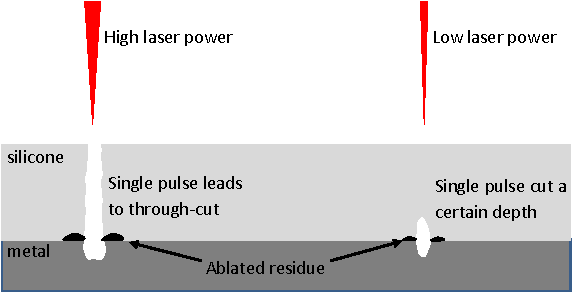
\includegraphics[width=0.6\textwidth]{figures/designandfabrication/figure3_21}%
\caption{Single laser pulse cut with high laser power and low laser power.}%
\label{figure3_21}%
\end{figure}

Since high laser power does not work for cutting silicone membrane with a certain depth, low laser power tests are conducted. As shown in \autoref{figure3_21}, with high laser power the most ablated metal particles generated by each laser pulse have the energy that is enough to penetrate the silicone membrane (these particles may have both high temperature and higher kinetic energy than that generated by low laser power). However, the energy of these metal particles will be significantly lowered down when the laser power decreases. And this energy is only enough to cut the silicone membrane a little bit each time. As a result, the cutting depth can be controlled simply by setting the processing passes. \\



Tests with low laser power are conducted with different numbers of processing passes. \autoref{figure3_22} shows the result pictures of the comparison of different processing passes taken from the LSM and SEM. From the 2 SEM pictures the cutting stripes can be observed. Picture (a) shows the result of 100 processing passes and the cutting depth is about 140$\mu$m calculated from the LSM profile. The SEM picture gives a sharply focused image of the processed area which is clean and flat and no through-cut holes present. The edge is a bit through-cut because the outline of the test square is cut for an extra time during each pass. Therefore the edge is cut for actually 200 passes and this problem is solved by excluding cutting the contour and does not present afterwards. Picture (b) shows the result of 85 processing passes and the cutting depth is about 100$\mu$m calculated from the LSM profile. Picture (c) shows the result of 70 processing passes.\\
\clearpage

\begin{figure}[!h]%
\centering
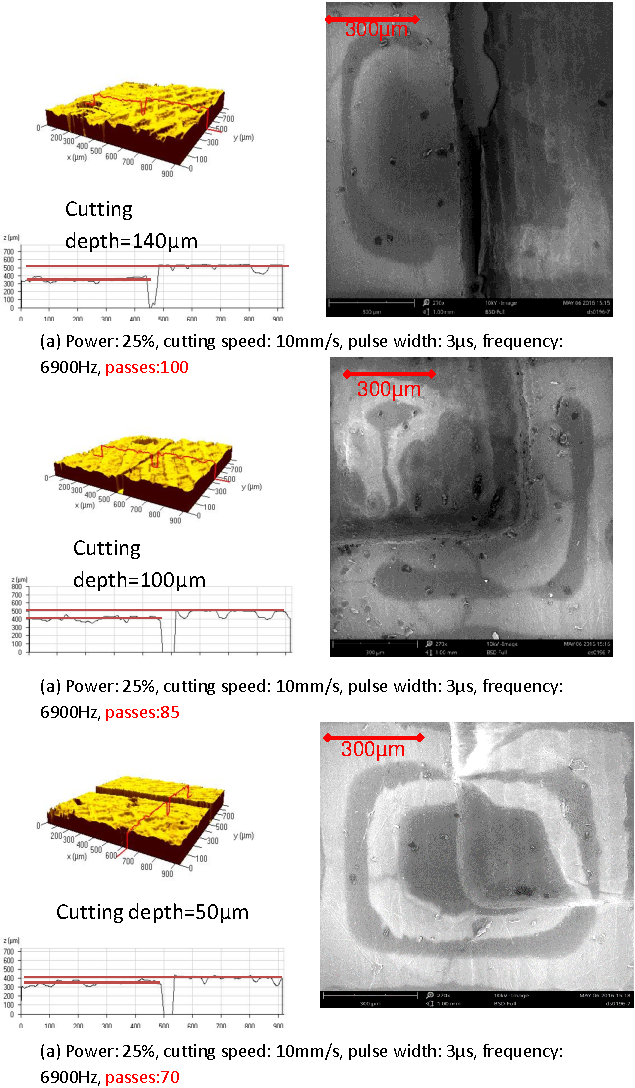
\includegraphics[width=0.82\textwidth]{figures/designandfabrication/figure3_22}%
\caption{Comparison of different processing passes with low laser power.}%
\label{figure3_22}%
\end{figure}

\clearpage

According to the data in the above Figure the cutting depth shows a linear relationship with the processing passes as shown in \autoref{figure3_22}. The linear equation is given as shown in \autoref{equation3_1}:

\begin{equation}
    d=3\times p-160
    \label{equation3_1}
\end{equation}

In this equation, d represents the cutting depth in micrometers and p represents the processing passes. However, this equation does not fit the calculation of cutting depth with low processing passes since it gives negative cutting depth with processing passes less than 50, which is impossible in reality. Therefore, the cutting depth is not correlated to the processing passes as shown in Equation 3.1 when the passes are low (at least less than 50). To characterize the relationship between the cutting depth and the processing passes with low passes, further tests need to be conducted and there might be different equations to fit to low numbers of passes, which is not done in this master thesis work.

\begin{figure}[ht]%
\centering
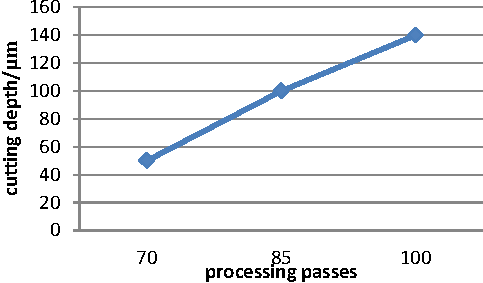
\includegraphics[width=0.55\textwidth]{figures/designandfabrication/figure3_23}%
\caption{Plot of the relationship between cutting depth and processing passes.}%
\label{figure3_23}%
\end{figure}

\begin{figure}[h]%
\centering
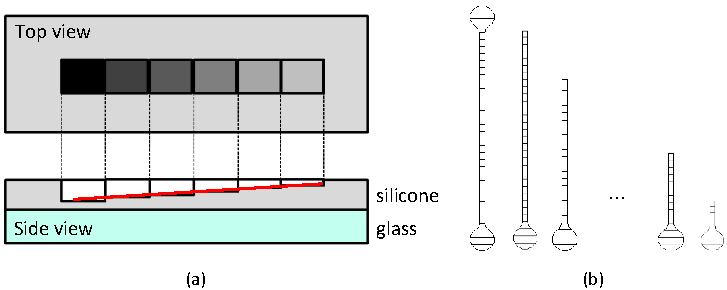
\includegraphics[width=0.8\textwidth]{figures/designandfabrication/figure3_24}%
\caption{(a) Steps with limited width can be regarded as gradual. (b) Processing mechanism of the microchannel.}%
\label{figure3_24}%
\end{figure}

\begin{figure}[!b]%
\centering
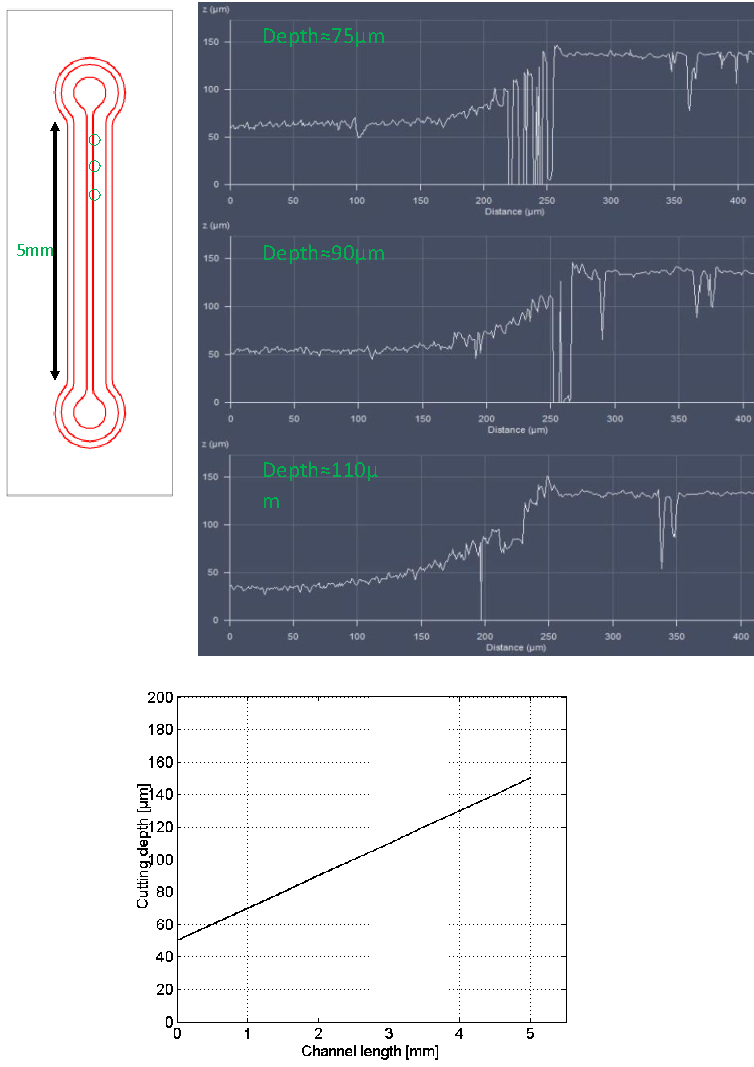
\includegraphics[width=0.9\textwidth]{figures/designandfabrication/figure3_25}%
\caption{Microchannel with variable depth.}%
\label{figure3_25}%
\end{figure}

Since it is already possible to machine microchannels with certain controllable depth in silicone membrane, a straight channel with gradual varying depth may be machined. This is done by defining steps along the length of the channel, as shown in \autoref{figure3_24} (a). In each of the step sections, the number of passes is varied, giving a varied cutting depth. If the step sections are kept relatively short, there will result a gradual continuous change in the channel height, because the laser patterning, especially by this indirect ablation method, does not yield perfect resolution.\\


\autoref{figure3_24} (b) shows the laser path to machine such channel. Firstly the total area, including the microchannel and the inlet and outlet reservoirs, is processed for 30 times as the base cycles. Then one reservoir and the microchannel are processed for 2 times as the step cycles. Afterwards the processed area is decreased gradually by decreasing 0.5mm channel length and the step cycles remain always 2. \autoref{figure3_25} shows the cutting depth measurement from the LSM.\\ 


From the figure above the change of the channel depth can be observed. The profiles are taken from different positions along the channel with the same reference plane. The channel depth varies along the channel from 75$\mu$m to 110$\mu$m. The depth of the inlet reservoir is 50$\mu$m and the depth of the outlet reservoir is 150$\mu$m. \autoref{figure3_25} shows depth profile from the start of the microchannel to the end of the microchannel and \autoref{figure3_26} shows the picture of the processed inlet reservoir and the channel.\\

\begin{figure}[ht]%
\centering
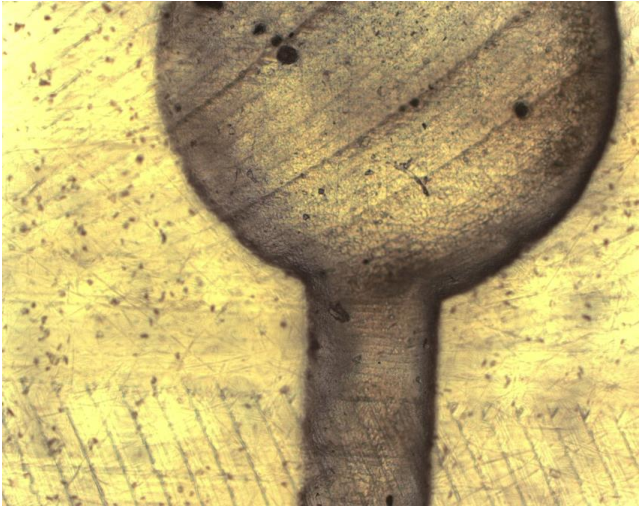
\includegraphics[width=0.6\textwidth]{figures/designandfabrication/figure3_26}%
\caption{Part of the microchannel with variable depth.}%
\label{figure3_26}%
\end{figure}

\clearpage

\section{Design and Fabrication of the Chip Housing}
\label{3_5}
The microfluidic platform in this thesis work is designed for testing the performance of the nanofiltration membrane and the adhesion and deposition features of bacteria on it. As shown in \autoref{figure3_27}, the silicone microchannel is designed for the suspension to flow through under high pressure. When the suspension flows over the nanofiltration membrane, it also permeates through the nanofiltration membrane which forms the permeate flow $Q_p$. The bacteria adhesion to the NF membrane should then be studied under the effect of this permeate flow. Furthermore, the shear stress along the channel length will change due to the change of channel depth and it is also of interest to study the contribution to the bacteria adhesion made by the shear stress. The initial housing design is to mount the silicone microchannel and keep it well sealed for the pressure and leakage test. Then the nanofiltration membrane need also be assembled into the housing. In this section, three designs are shown. The first design is simply to test the pressure bearing capacity of the silicone microchannel. The second design is improved based on the first design. The third design is the final housing design containing the nanofiltration membrane, which required a modification of the inlet and outlet configuration.\\

\begin{figure}[ht]%
\centering
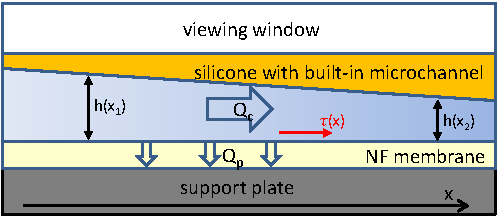
\includegraphics[width=0.6\textwidth]{figures/designandfabrication/figure3_27}%
\caption{Design concept of the microfluidic platform}%
\label{figure3_27}%
\end{figure}

\subsection{Housing Design 1}
\label{3_5_1}
In this design the fluid flows simply through the microchannel under high pressure. The fluid is pressurized by a pressure accumulator which is illustrated in \autoref{3_6}. The housing must be able to withstand high pressure at least up to 10bar. The glass slide, as the mechanical carrier of the silicone membrane, must also remain intact under such pressure and the fluid should not leak to anywhere other than the microchannel.

\begin{figure}[!h]%
\centering
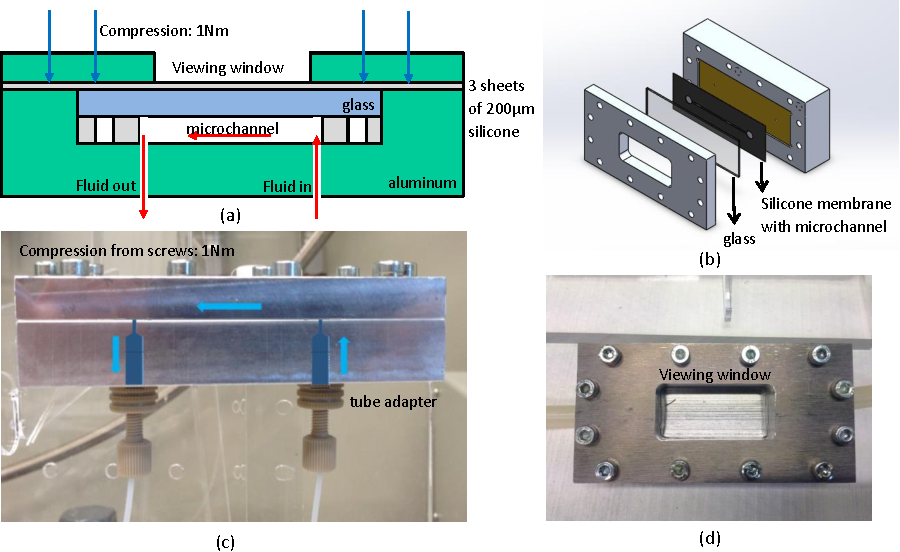
\includegraphics[width=1\textwidth]{figures/designandfabrication/figure3_28}%
\caption{Schematic of the housing design 1 and the finished product. (a) Side view of the schematic of the housing design. (b) Isometric view of the assembly of the housing design. (c) Side view of the finished product. (d) Top view of the finished product.}%
\label{figure3_28}%
\end{figure}

As we can see in \autoref{figure3_28} the silicone membrane together with the glass slide is pressed against the base plate of the housing. In this way the microchannel is sealed by the seamless contact between the silicone membrane and the base plate. The inlet and the outlet are placed at the bottom side so that fluid can directly enter the microchannel. A metal lid is connected to the base plate by 12 screws to provide compression to the glass slide for sealing. However, in this case the compression lies on the four edges of the glass slide and the center of the glass slide is not compressed, resulting in a non-uniform distributed compression force. To avoid direct contact of the metal lid and the glass slide and also to achieve a more evenly compression distribution, 3 layers of silicone membranes are placed in between to provide a cushion room since metal and glass are both rigid materials. There is a window in the middle of the metal lid in order to observe the microchannel from the top side. The screws are tightened by the torque wrench and the torque is set to 1N$\cdot$m.

\subsection{Housing Design 2}
\label{3_5_2}
\begin{figure}[t]%
\centering
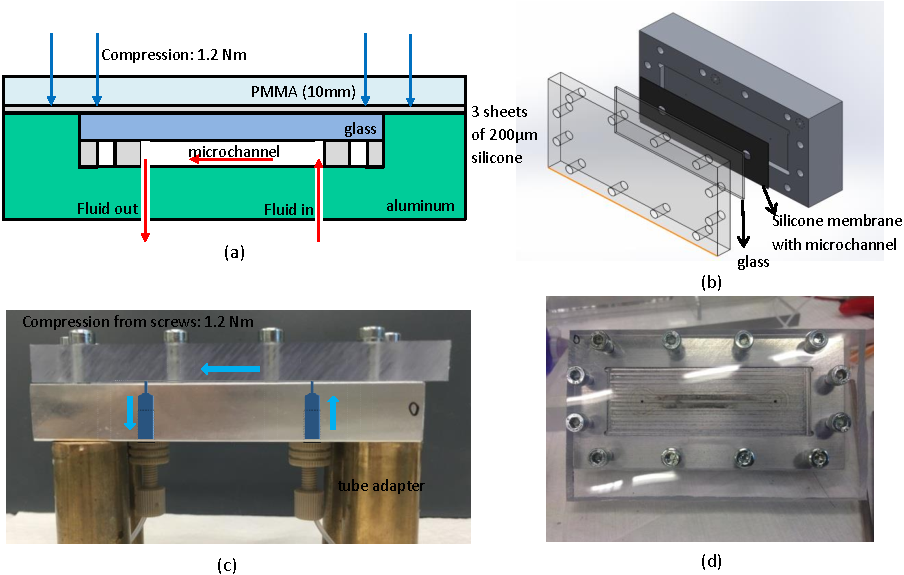
\includegraphics[width=1\textwidth]{figures/designandfabrication/figure3_29}%
\caption{Schematic of the housing design 2 and the finished product. (a) Side view of the schematic of the housing design. (b) Isometric view of the assembly of the housing design. (c) Side view of the finished product. (d) Top view of the finished product.}%
\label{figure3_29}%
\end{figure}

In the former housing design the lid is made from aluminum and the viewing window is in the middle of this lid. The glass slide is pushed against the base plate by the metal lid. However, the force bearing area on the glass slide is at the four edges, and that leads to a non-uniform force distribution. Therefore the glass slide broke easily when the screws were tightened and even though it was successfully assembled, cracks appeared at the inlet and outlet at the pressure of only 1 bar. Moreover, the viewing window is also not large enough to show the whole channel and the inlet and outlet reservoirs.\\

To solve these problems, the aluminum lid is replaced by a PMMA lid. Since PMMA is totally transparent, it needs not to be cut in the middle for the viewing window and this time a full view of the microchannel can be achieved. Another advantage of using PMMA lid is that the glass slide is in full contact with the lid so that the compression force distribution is quite uniform over the full slide surface. Hence the glass slide will not break easily. \autoref{figure3_29} shows the schematic design and the finished product of housing design 2.

\subsection{Housing Design 3}
\label{3_5_3}
\begin{figure}[t]%
\centering
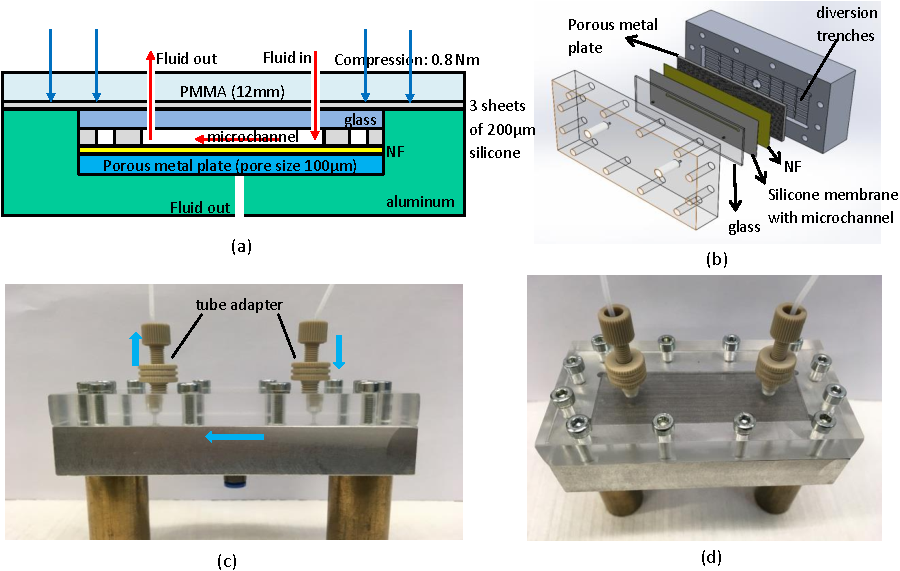
\includegraphics[width=1\textwidth]{figures/designandfabrication/figure3_30}%
\caption{Schematic of the housing design 3 and the finished product. (a) Side view of the schematic of the housing design. (b) Isometric view of the assembly of the housing design. (c) Side view of the finished product. (d) Top view of the finished product.}%
\label{figure3_30}%
\end{figure}

The former designs are targeted at testing the highest pressure that the microchannel can withstand so that the NF membrane is not taken into account. In this design, the aim is to assemble all the parts including the microchannel and the NF membrane inside. \\

\autoref{figure3_30} (a) shows the schematic design. The silicone membrane with built in microchannel sits on top of the NF membrane so that the fluid can flow over the NF membrane. Since the thickness of the NF membrane is only 160$\mu$m and it can deform easily, a support plate need to be placed underneath. This support metal plate is made of stainless steel and is porous so that the fluid which permeates the NF membrane could flow out through the outlet hole at the bottom of the housing. The pore size of the porous metal plate is 100$\mu$m and water can permeate this plate with minimal resistance.\\

In this housing design the fluid should not be loaded in to the channel from the bottom side since the NF membrane needs to be intact and sealed against the silicone gasket. As a result, the inlet and outlet interfaces are placed at the top side. The PMMA lid is drilled with threaded holes to assemble the tube adapters as shown in \autoref{figure3_30} (c). Two holes for the inlet and outlet are also drilled in the glass slide to let the fluid flow through. The diameter of these two holes is 1.1mm. There are also interlaced diversion trenches designed beneath the porous metal plate in the aluminum housing to let the permeated fluid to flow out as shown in \autoref{figure3_30} (b). \autoref{figure3_30} (c) and (d) show the finished product of the design.\\ 

For drilling the inlet and outlet holes in the glass slide was to build a stack of glass slides. The chip (glass slide with the patterned silicone membrane) is covered by two layers of sacrificial glass slides of the same size as shown in \autoref{figure3_31} (a). This stack is fixed by colophony, which melts at 120$^\circ$C and solidifies at room temperature, so that the glass slides will not move during drilling. Then the colophony is removed from the stack and the chip is taken out and cleaned by ethanol (colophony dissolves in ethanol).

\begin{figure}[!t]%
\centering
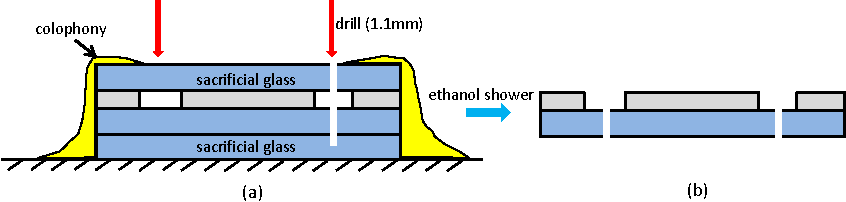
\includegraphics[width=1\textwidth]{figures/designandfabrication/figure3_31}%
\caption{Glass drilling process. (a) The chip is covered by two sacrificial glass slides and fixed by colophony. (b) Colophony is cleaned by ethanol.}%
\label{figure3_31}%
\end{figure}

\begin{figure}[!t]%
\centering
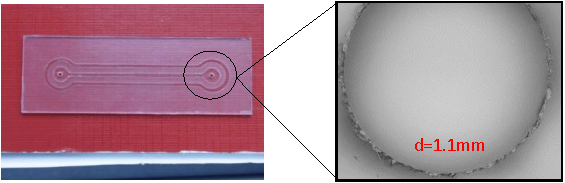
\includegraphics[width=0.7\textwidth]{figures/designandfabrication/figure3_32}%
\caption{Microscopic view of the drilled holes in glass slide.}%
\label{figure3_32}%
\end{figure}
\autoref{figure3_32} shows the microscopic view of the holes in the glass slide. The glass slide does not break during the drilling process and no cracks present as well.

\clearpage

\section{Design of the Test Setup}
\label{3_6}
As discussed in previous sections, the main goal is to test the working performance of the microchannel and the NF membrane under high pressure. In this section, the test setup is designed to pressurize the fluid and load it into the microchannel.\\

A pressure accumulator is designed to pump fluid into the microfluidic platform as shown in \autoref{figure3_33}. The pressure accumulator is made of aluminum and it has a wall thickness of 18.82mm. It is sealed by 6 O-rings, 2 O-rings used for the movable piston to separate the nitrogen and loaded water and 4 O-ring used to seal the both lids. In this way the high pressure nitrogen gas can be used to pressurize the housing. 

\begin{figure}[ht]%
\centering
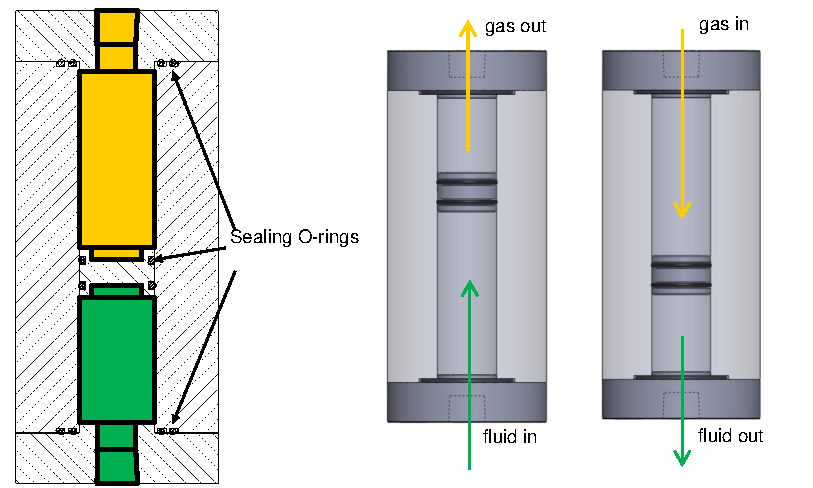
\includegraphics[width=0.8\textwidth]{figures/designandfabrication/figure3_33}%
\caption{Schematic and working principle of the pressure accumulator.}%
\label{figure3_33}%
\end{figure}

\autoref{figure3_34} shows the schematic design of the test setup with housing design 2. A pressure regulator with a relief valve set at 50bar is used to apply pressure to a piston in the pressure accumulator, which drives the flow into the microchannel. A syringe is connected to the canister and the piston will be pushed upwards to load fluid into the canister. Two pressure sensors (PS) with accuracy of 0.6bar are installed to measure both, the fluid pressure before it enters the microchannel and the fluid pressure it flows out of the microchannel. The measurements are made every 1ms and the data acquisition device (NI-USB 6008 from National Instruments) transfers the pressure measurements to a PC, where the data is analyzed and stored. A back pressure regulator (BPR) is also installed to keep the pressure inside the microchannel to a set value.\\
\clearpage
\begin{figure}[ht]%
\centering
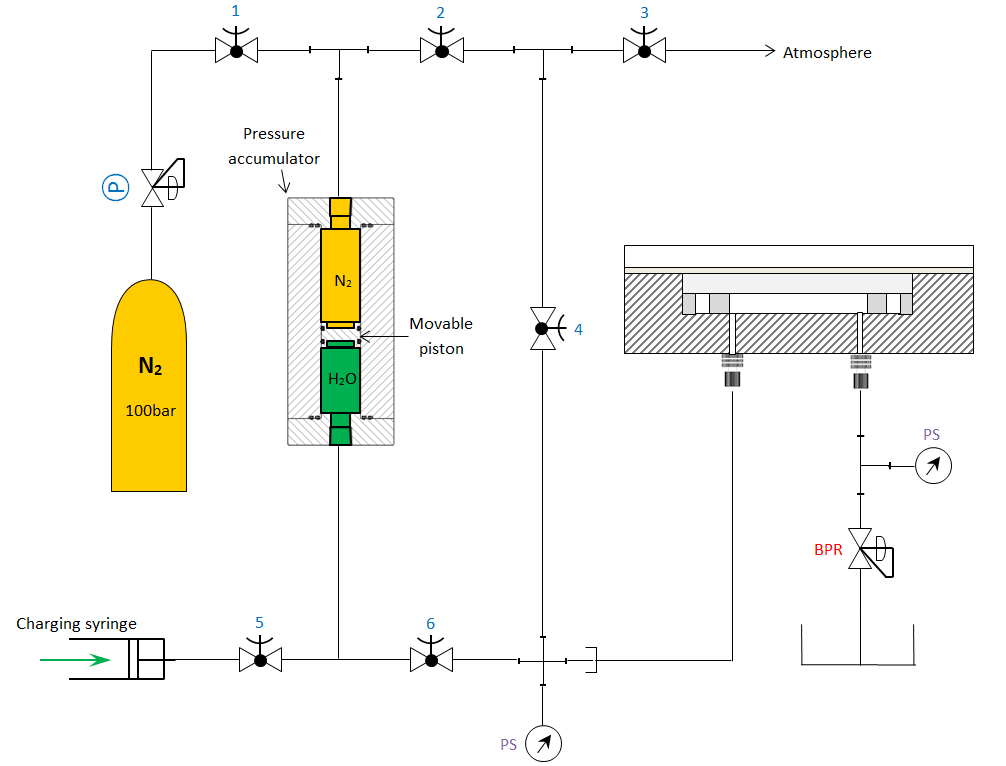
\includegraphics[width=1\textwidth]{figures/designandfabrication/figure3_34}%
\caption{Schematic of the test setup design.}%
\label{figure3_34}%
\end{figure}



\noindent \textit{Loading fluid to the pressure accumulator}\\

Consider that all the valves are closed. By opening the valves 2, 3 and 5 the fluid can be pre-loaded into the pressure accumulator. This is done by using a syringe coupled to valve 5 and by pushing the syringe the movable piston will be pushed upwards, repelling the gas out of the canister and thus fluid is loaded as shown in \autoref{figure3_35}. Once the fluid is loaded to the pressure accumulator, the valve 2, 3 and 5 must be closed in order to keep the fluid inside the system.\\
\clearpage

\begin{figure}[ht]%
\centering
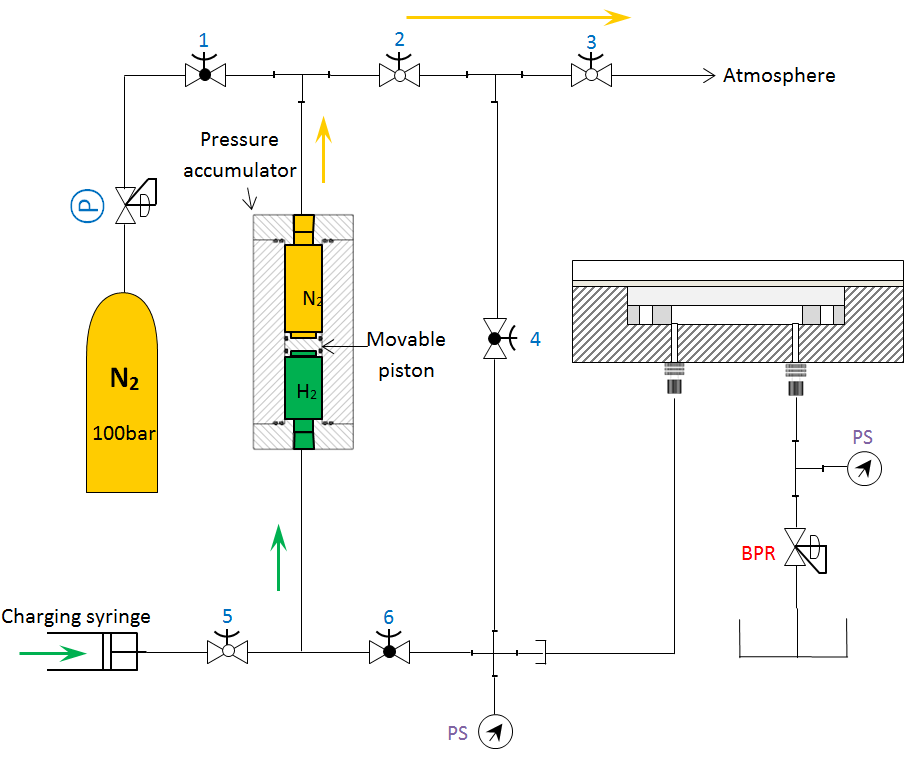
\includegraphics[width=0.8\textwidth]{figures/designandfabrication/figure3_35}%
\caption{Loading fluid into the pressure accumulator.}%
\label{figure3_35}%
\end{figure}

\noindent \textit{Pumping the fluid into the microfluidic platform}\\

Consider that all the valves are closed. By opening the valves 1 and 6 the nitrogen will flow from the high pressure nitrogen tank to the pressure accumulator and cause downward displacement of the piston, which pumps the fluid into the microfluidic platform. Since the BPR only releases pressure when the pressure is higher than its set value, the pressure regulator at the high pressure nitrogen tank should be set at a pressure higher than the BPR can withstand.\\
\clearpage

\begin{figure}[ht]%
\centering
\includegraphics[width=0.8\textwidth]{figures/designandfabrication/figure3_36}%
\caption{Pumping the fluid into the microfluidic platform.}%
\label{figure3_36}%
\end{figure}

\noindent \textit{Purging the microchannel}\\

Consider that all the valves are closed. By opening the valves 1, 2 and 4 the nitrogen will flush into the microchannel and thus the flow loop is purged.\\
\clearpage

\begin{figure}[!h]%
\centering
\includegraphics[width=0.8\textwidth]{figures/designandfabrication/figure3_37}%
\caption{Purging the microchannel.}%
\label{figure3_37}%
\end{figure}





\chapter{Packaging and Tests under High Pressure}
\label{4}
In this chapter, packaging of both the chip housing and the test setup is presented. To start with, the packaging of the test setup is presented and an array of pressure accumulators is used, to increase stored fluid volume over the single canister shown in \autoref{3_6}. Then a preliminary chip housing design without integrating the NF membrane is introduced, followed by the second housing design which is improved based on the first design. The final housing design provides the possibility to integrate NF membrane. Therefore the positions of the inlet and outlet interfaces are changed and an additional supporting plate is introduced as the mechanical carrier of the NF membrane. At last the pressure and leakage test results and some calculation with respect to the flow parameters in the microchannel are presented.

\section{Packaging of the Test Setup}
\label{4_1}
In \autoref{3_6} the design of the test setup is presented. Since the system will be pressurized up to 10bar, all the connection interfaces and tubes should be able to withstand such high pressure. Therefore the adapters and connectors connecting to the pressure accumulator are made of metal (either brass or stainless steel (SS)). The chip housing is connected to this test setup by adapters and fittings made of PEEK and ETFE tubes which are designed for high pressure applications (up to 69bar). \autoref{figure4_1} shows the schematic design of all the connections and \autoref{figure4_2} shows the real packaging of the test setup and \autoref{table4_1} gives the name of the used parts, their material and the maximum pressure they can withstand.\\
\clearpage

\begin{figure}[h]%
\centering
\includegraphics[width=0.82\textwidth]{figures/packagingandtestunderhighpressure/figure4_1}%
\caption{Schematic design of the test setup packaging with housing design 2 introduced in \autoref{3_5_2}.}%
\label{figure4_1}%
\end{figure}

\begin{table}[!h]
    \centering
    \caption{Used parts and their material and maximum working pressure}
    \begin{longtable}{l|l|l|l|l}
    \toprule
    No. & Name & Material & Pressure (bar) & Supplier \\
    \midrule
    1 & Needle valve & Brass & 206 & Swagelok \\
    2 & Plug valve & Brass & 206 & Swagelok \\
    3 & Tee & Brass & 248 & Swagelok \\
    4 & Cross & Brass & 248 & Swagelok \\
    5 & Tube fitting & Brass & 275 & Swagelok \\
    6 & Tubing & SS & 351 & Swagelok \\
    7 & Tube fitting & Brass & 227 & Swagelok \\
    8 & Connector & Brass & 227 & Swagelok \\
    9 & Connector & SS & 551 & Swagelok \\
    10 & Connector & Brass & 275 & Swagelok \\
    11 & Fitting & Brass & 275 & Swagelok \\
    12 & Pressure sensor &   & 0-250 & Gems \\
    13 & Adapter & PEEK & 69 & IDEX \\
    14 & Tube fitting & PEEK & 414 & IDEX \\
    15 & Tubing & ETFE & 207 & IDEX \\
    \bottomrule
    \end{longtable}
    \label{table4_1}
\end{table}
\clearpage

\begin{figure}[!h]%
\centering
\includegraphics[width=0.6\textwidth]{figures/packagingandtestunderhighpressure/figure4_2}%
\caption{Practical packaging of the test setup and connection to the chip housing.}%
\label{figure4_2}%
\end{figure}

\autoref{figure4_3} shows the dimensions of the interior space of the pressure accumulator. The total usable volume that can be loaded is calculated to be 34.9mL according to these dimensions. However, such volume is not enough for continuous long-time (at least 30min) flow test since the volume flow rate is around 5mL/min as initial tests indicated. Therefore the pressure accumulator is redesigned to a canister array which contains six canisters instead of only one canister that was used before. The total available volume is expanded to about 210mL. \\

In the new design the six canisters stand on a holder. All the connectors, tube fittings and valves are made of brass and the metal tube is made of stainless steel. Therefore the maximum pressure this system can withstand is more than 200bar and this ensures the safety since the test in this thesis work is around 10bar. \autoref{figure4_4} shows the design and connection of the canister array.\\

\begin{figure}[ht]%
\centering
\includegraphics[width=0.5\textwidth]{figures/packagingandtestunderhighpressure/figure4_3}%
\caption{Dimensions of the pressure accumulator and the canister array.}%
\label{figure4_3}%
\end{figure}

\begin{figure}[ht]%
\centering
\includegraphics[width=1\textwidth]{figures/packagingandtestunderhighpressure/figure4_4}%
\caption{Design and connection of the canister array.}%
\label{figure4_4}%
\end{figure}
\clearpage


\section{Packaging and Pressure Test of the Microfluidic Platform Housing}
\label{4_2}
\subsection{Packaging Requirements}
\label{4_2_1}
Since the goal of this thesis work is to design a reusable and resealable microfluidic platform, the first task is to design a good packaging interface that fulfills the following requirements: reusability, resealability, easy manipulation, flexibility and fast connectivity. Besides, because this microfluidic platform is supposed to work under high pressure, it must provide reliable sealing (no leakage at high pressures) and mechanical stability (able to work at high pressures). Since the microfluidic platform should be assembled and disassembled for many times in order to test with different microchannel designs and different NF membranes with the same chip, the packaging must be adhesive-free as well.\\

One other important specification is the ability to have good visual access to the microchannel inside the housing. This is critical to the microfluidic platform because direct observation of the bacteria adhesion to the NF membrane surface is desired. A live monitoring of the bacteria is not only helpful to characterize the adhesion features under specific flow conditions, but also provides information about how to change the real-time flow conditions to control the adhesion heading for a certain direction (similar to closed-loop control). 

\subsection{Packaging and Pressure Test of Different Chip Housing Design}
\label{4_2_2}
\noindent \textit{Packaging of the housing design 1}\\

\begin{figure}[h]%
\centering
\includegraphics[width=0.95\textwidth]{figures/packagingandtestunderhighpressure/figure4_5}%
\caption{Schematic of the housing assembly (design 1).}%
\label{figure4_5}%
\end{figure}

The first design consists of an aluminum housing, glass slide with silicone membrane which has built-in microchannel, a cushion silicone membrane, macro-to-micro adapters and 12 screws (M4).\\

\begin{figure}[h]%
\centering
\includegraphics[width=0.7\textwidth]{figures/packagingandtestunderhighpressure/figure4_6}%
\caption{Explosion view of the housing assembly and packaged housing assembly.}%
\label{figure4_6}%
\end{figure}

\autoref{figure4_5} shows the schematic of the housing assembly. The inlet and outlet interfaces are at the bottom of the support plate, coupled with adapters and tube fittings from IDEX. The fluid enters the microchannel through an orifice which has a diameter of 1mm and this orifice is sealed by the glass slide and the surrounding silicone gasket. The connecting tube is made of ETFE and has an out diameter of 1/16inch (1.5875mm) and inner diameter of 0.02inch (0.5mm). A cavity in the support plate is designed for the location and the alignment of the glass slide and silicone membrane. There is an aperture machined in the center of the lid and it works as a window for visual access to the microchannel. \\

Before the packaging is started, the cavity in the aluminum support plate, the silicone membrane, the glass slide and the silicone cushion membrane need to be cleaned by ethanol to remove the dust at surfaces as much as possible.  Then the microchannel and the carrier glass slide are placed into the cavity in the support plate and are aligned to the cavity, after which three layers of cushion silicone membrane (3$\times$200$\mu$m) are placed in between the lid and the support plate in order to prevent damaging the glass slide by avoiding direct metal-glass contact since glass is rigid and fragile material. Finally the lid is joined to the support plate by twelve M4 screws and four edges of the glass slide are compressed by the lid as shown in \autoref{figure4_6}.\\


\noindent \textit{Test results and evaluation of housing design 1}\\

\begin{figure}[!b]%
\centering
\includegraphics[width=0.6\textwidth]{figures/packagingandtestunderhighpressure/figure4_7}%
\caption{(a) Cracks appeared during the packaging. (b) Crack appeared when pressurized up to 1bar.}%
\label{figure4_7}%
\end{figure}

Before pressure test all the screws are tightened. Then the outlet interface is plugged to hold the pressure inside the microchannel. The microchannel should withstand each test pressure for at least 10min in order to test the long-term stability. Furthermore, any leakage will also be checked.\\

The screws were tightened stepwise with increasing torque, using a star pattern to ensure loading remained as evenly distributed as possible. By tightening the screws different torque values were tried (2N$\cdot$m, 1.5N$\cdot$m, 1N$\cdot$m). However, as shown in \autoref{figure4_7} (a), cracks appeared in the glass slide when the torque is set to 2N$\cdot$m and 1.5N$\cdot$m. Even though the glass slide remained intact at 1N$\cdot$m tightening torque, it broke at the inlet interface when the pressure reached 1bar as presented in \autoref{figure4_7} (b). \\

The cracks appeared in the glass slide during tightening the screws because of the uneven compression force to the glass slide. Since the center part of the glass slide is not covered by the aluminum lid because of the viewing window, the compression force distributes only to the four edges of the glass slide, leading to an uneven force distribution. Therefore even no cracks appear during assembling the housing, it will bring more risk when it is working under high pressure.\\

Another drawback of this housing design is the limited view of the microchannel. Since the viewing window in the lid is relatively small, the inlet and outlet interfaces are covered by the lid. Therefore for a better visual access to the microchannel the lid should be redesigned.\\

\noindent \textit{Packaging of the housing design 2}\\

\begin{figure}[!b]%
\centering
\includegraphics[width=1\textwidth]{figures/packagingandtestunderhighpressure/figure4_8}%
\caption{Schematic of the housing assembly (design 2).}%
\label{figure4_8}%
\end{figure}

In the second chip housing design the aluminum lid is replaced by a PMMA lid while the other parts remain the same. Since PMMA has excellent optical transparency, the whole microchannel can be viewed from the top side. Furthermore, no window aperture is needed in the lid so that the PMMA lid is in full contact with the glass slide, which provides a homogeneous force distribution to the glass slide surface. \autoref{figure4_8} shows the schematic of the chip housing assembly, the packaging procedure is the same to the first design. The silicone microchannel, the glass slide together with the silicone cushion membrane and the PMMA lid need to be cleaned before packaging because any uneven points at the surfaces can cause failure of the glass slide, and this damage can be amplified especially by the high pressure.\\

\noindent \textit{Test results and evaluation of housing design 2}\\

The torque applied to the screws was set to 1.2N$\cdot$m and no cracks presented during the packaging of the housing. This is because the force distribution is even at the glass slide surface. Then the pressure was applied to the microchannel gradually, starting from 1bar with a step of 0.2bar.  One crack appeared at the outlet interface when the pressure reached 3.4bar as shown in \autoref{figure4_9} (a). 

\begin{figure}[!h]%
\centering
\includegraphics[width=0.6\textwidth]{figures/packagingandtestunderhighpressure/figure4_9}%
\caption{(a) Crack appeared at 3.4bar with screw torque of 1.2N$\cdot$m. (b) No crack appeared when loaded to 8bar with screw torque of 1N$\cdot$m.}%
\label{figure4_9}%
\end{figure}

Then the torque applied to the screws was lowered to 1N$\cdot$m in the next experiment. Likewise, no cracks in the glass slide presented during packaging. The microchannel was pressurized up to 8bar for two times and for each time it stayed at 8bar for 30min. Finally the glass slide remained intact as shown in \autoref{figure4_9} (b). This indicates that silicone microchannel with glass slide as its mechanical carrier can seal well by compression and is able to work under high pressure.

\noindent \textit{Packaging of the housing design 3}\\

\begin{figure}[h]%
\centering
\includegraphics[width=1\textwidth]{figures/packagingandtestunderhighpressure/figure4_10}%
\caption{Schematic of the housing assembly (design 3).}%
\label{figure4_10}%
\end{figure}

In the third housing design the NF membrane is taken into account. Since the NF membrane should be intact to ensure valid filtration, the inlet and outlet interfaces are placed in the PMMA lid. In this case the permeate flow is introduced by the filtration performance of the NF membrane. Therefore a porous support plate is placed under the NF membrane and several trenches are designed underneath the porous support plate to collect the permeate flow. A single layer of 600$\mu$m silicone cushion membrane is placed in between the lid and the housing support instead of three layers of 200$\mu$m thick membranes.  \autoref{figure4_10} shows the schematic of the chip housing assembly. The packaging procedure is the same to the prior designs.\\

\noindent \textit{Test results and evaluation of housing design 3}\\

For pressure and leakage test the NF membrane is not initially applied. A piece of stainless steel of the same thickness was placed instead of the NF membrane. \autoref{figure4_11} shows the packaged housing with microchannel integrated inside. Likewise, no crack presented when the tightening torque is 1N$\cdot$m and it worked stably under high pressure (8bar).\\
\clearpage

\begin{figure}[h]%
\centering
\includegraphics[width=0.6\textwidth]{figures/packagingandtestunderhighpressure/figure4_11}%
\caption{Packaged housing of design 3.}%
\label{figure4_11}%
\end{figure}

\section{Hydrodynamic Characterization of the Microchannel}
\label{4_3}
As presented in \autoref{4_2}, housing design 3 provides a stable performance working under high pressure and also offers the possibility to integrate NF membrane into the housing. Therefore the hydrodynamic characterization tests of the microchannel are done with housing design 3 and \autoref{figure4_12} shows the schematic of the test setup.\\

Two pressure sensors are integrated to the flow path to measure the fluid pressure before it enters the microchannel and after it leaves the microchannel. In the following tests the total pressure drop is achieved by calculating the pressure difference measured by these two pressure sensors. Therefore this total pressure drop is consisted of the pressure drop in the tube through which fluid enters the chip housing, the pressure drop in the microchannel and the pressure drop in the tube which connects the outlet of the chip housing and the second pressure sensor. The pressure sensor is a current output transducer which has a measuring range from 0 to 250bar. \\
\clearpage

\begin{figure}[h]%
\centering
\includegraphics[width=0.85\textwidth]{figures/packagingandtestunderhighpressure/figure4_12}%
\caption{Schematic of the test setup with housing design 3.}%
\label{figure4_12}%
\end{figure}

\subsection{Calibration of the Pressure Sensor}
\label{4_3_1}
The pressure sensor is calibrated before use. Since the output of the pressure sensor is current with respect to the pressure and the available data acquisition (DAQ) NI-6008 USB device in our lab can only measure analog voltage, a resistor of 1k$\ohm$ is connected to the pressure sensor as shown in \autoref{figure4_13}. The pressure sensor is powered by a voltage source with a voltage of 30V. In this way the output current is converted to voltage and this voltage is estimated to be in the range of 4V to 5V. Since the analog-to-digital converter (ADC) in the DAQ device might also consume part of current for the measurement of the voltage between both sides of the resistor, possible disturbance might be introduced if the DAQ device is connected directly in parallel to the resistor and takes part of the current that should flow through the resistor. Therefore, an operational amplifier which is connected as a voltage follower is placed as a barrier between the resistor and the DAQ module since it consumes nearly no current at the input side because of its large input resistance. Moreover, the voltage between the two sides of the resistor is precisely transferred to the DAQ module since the very low output resistance of the operational amplifier does not consume this voltage. The sample rate of the DAQ module is set to 1k, indicating that 1000 samples will be sent to the computer via USB cable within one second. The Labview program in the computer receives the data and calculates the average value of every 1000 pressure data, resulting in a relatively more stable and precise output display in the user interface. Two channels of analog voltage input port are used for the two pressure sensors. 

\begin{figure}[h]%
\centering
\includegraphics[width=0.9\textwidth]{figures/packagingandtestunderhighpressure/figure4_13}%
\caption{Electrical connections for pressure measurement}%
\label{figure4_13}%
\end{figure}

The calibration pressure starts from 1 bar to 7bar with a step of 0.5bar. The measured voltage corresponding to the pressure is listed in \autoref{table4_2}. Based on this acquired data linear regression is done to figure out the linear relation between pressure and measured voltage. \autoref{figure4_14} shows the results graph of the linear regression and the linear equation is given below:

\begin{table}[!h]
    \centering
    \caption{Measured voltage and the corresponding pressure}
    \begin{tabular}{cc}
    \toprule
    Pressure (bar) & Measured Voltage (V) \\
    \midrule
    1 & 4.05\\
    1.5 & 4.09\\
    2 & 4.11\\
    2.5 & 4.15\\
    3 6 & 4.18\\
    3.5 & 4.21\\
    4 & 4.24\\
    4.5 & 4.27\\
    5 & 4.31\\
    5.5 & 4.34\\
    6 & 4.37\\
    6.5 & 4.40\\
    7 & 4.44\\
    \bottomrule
    \end{tabular}
    \label{table4_2}
\end{table}

\begin{figure}[!h]%
\centering
\includegraphics[width=0.6\textwidth]{figures/packagingandtestunderhighpressure/figure4_14}%
\caption{Linear regression of the voltage and pressure.}%
\label{figure4_14}%
\end{figure}

\begin{equation}
    V=63.45 \cdot P+3993
    \label{equation4_1}
\end{equation}

\begin{equation}
    R^2=0.9997
    \label{equation4_2}
\end{equation}

where V is the measured voltage (mV) and P is the corresponding pressure (bar). Since the coefficient of determination, $R^{2}$, is very close to 1, the linearity between voltage and pressure is good enough. According to the \autoref{equation4_1} pressure can be calculated with respect to the measured voltage as shown in \autoref{equation4_3}. For the following tests the pressure (P) is calculated according to \autoref{equation4_3} by Labview and saved.

\begin{equation}
    P=\frac{V-3993}{63.45}
    \label{equation4_3}
\end{equation}

\subsection{Cross Flow Rate Measurement}
\label{4_3_2}

\begin{figure}[!b]%
\centering
\includegraphics[width=0.6\textwidth]{figures/packagingandtestunderhighpressure/figure4_15}%
\caption{Microchannel geometry under test.}%
\label{figure4_15}%
\end{figure}

To characterize the hydrodynamic parameters of the microchannel, the cross flow rate under different pressures is measured and the pressure difference between the two pressure sensors is also calculated. \autoref{figure4_15} shows the microchannel geometry under test. No permeation flow is introduced and the NF membrane is replaced by a piece of steel sheet in this test.\\



The fluid loading in the system in this test is water. The flow rate is measured by recording the time for collecting 5mL water at the outlet interface after the back pressure regulator. \autoref{figure4_16} shows the pressure profile recorded by Labview, including the pressure data from the two pressure sensors and the pressure difference of the two pressure sensors. \autoref{table4_3} shows the measured pressures before and after the microchannel and the calculated volume flow rate:

\begin{figure}[ht]%
\centering
\includegraphics[width=0.8\textwidth]{figures/packagingandtestunderhighpressure/figure4_16}%
\caption{Recorded pressure data from Labview.}%
\label{figure4_16}%
\end{figure}

\autoref{figure4_17} shows the plot of total pressure drop and the flow rate in the channel versus the pressure at inlet interface. The flow rate in the channel shows good linearity with respect to the input pressure and this means the flow rate can be estimated by controlling the input pressure.\\
\clearpage

\begin{table}[!h]
    \centering
    \caption{Pressure data and corresponding volume flow rate.}
    \begin{tabular}{C{2.3cm} C{2.3cm} C{2.3cm} C{2.5cm} C{2.2cm}}
    \toprule
    Inlet Pressure (bar) & Outlet Pressure (bar) & Pressure Drop (bar) & Time for 5mL Collection (s) & Volume Flow Rate (mL/min) \\
    \midrule
    7.35 & 6.85 & 0.5 & 95 & 3.1579\\
    7.8 & 7.1 & 0.7 & 69 & 4.3478\\
    8.08 & 7.24 & 0.85 & 57 & 5.2632\\
    8.25 & 7.3 & 0.95 & 52 & 5.7692\\
    8.64 & 7.5 & 1.14 & 42 & 7.0588\\
    9.35 & 7.75 & 1.6 & 33 & 9.0909\\
    9.98 & 7.9 & 2.08 & 27 & 11.1111\\
    10.8 & 8.15 & 2.65 & 22 & 13.6364\\
    11.5 & 8.3 & 3.2 & 19 & 15.7894\\
    \bottomrule
    \end{tabular}
    \label{table4_3}
\end{table}

\begin{figure}[!h]
\centering
\subfigure{\includegraphics[width=0.48\textwidth]{figures/packagingandtestunderhighpressure/figure4_17a.pdf}}
\centering
\subfigure{\includegraphics[width=0.48\textwidth]{figures/packagingandtestunderhighpressure/figure4_17b.pdf}}
\centering
\caption{(a) Total pressure drop versus pressure at inlet. (b) Volumetric flow rate in the microchannel versus total pressure drop.}
\label{figure4_17}%
\end{figure}

\noindent \textit{Fluidic system modeling}\\

As shown in \autoref{figure4_18} (a), there are three segments between the two pressure sensors: the tube through which fluid reaches the inlet of the chip housing, the microchannel in the housing and the tube connecting the outlet of the housing to the second pressure sensor. The pressure difference between the two pressure sensors therefore contains respective pressure drop in these three segments. An analogy to electrical circuits may be made, in which the total pressure drop is regarded as a voltage source while the flow rate is regarded as current. Likewise, each segment tube and the microchannel have their own fluidic resistances. \autoref{figure4_18} (b) presents the corresponding electric circuit representing this hydrofluidic system. \autoref{equation4_4} gives the Ohm's law in hydrodynamics:

\begin{equation}
    \Delta P=I_V\cdot R
    \label{equation4_4}
\end{equation}

In the equation above, $\Delta$P is the pressure drop measured by the two pressure sensors, $I_V$ is the volume flow rate which represents current in electric circuits and R is the fluidic resistance. For laminar flow in the tubes with circular cross-section the flow rate can be calculated according to Hagen-Poiseuille-Law \cite{hpequation}:

\begin{equation}
    I_V=\frac{\pi r^4}{8\eta} \frac{\Delta P}{l}
    \label{equation4_5}
\end{equation}

Where r is the inner diameter of the tube, $\eta$ is the dynamic viscosity of the fluid, $\Delta$P is the pressure drop and l is the length of the tube. Therefore the fluidic resistance of the tube is given by \autoref{equation4_6}:

\begin{equation}
    R_{circle}=\frac{8\eta l}{\pi R^4}
    \label{equation4_6}
\end{equation}

The dynamic viscosity of water at room temperature is given \cite{waterviscosity}:

\begin{equation}
    \eta (water)=890\times 10^{-6} Pa\cdot s
    \label{equation4_7}
\end{equation}

The fluidic resistance of rectangular cross-section microchannel under laminar flow is given by the following equation \cite{fuerstman2007pressure}:

\begin{equation}
    R_{rechtangle} = \frac{12\eta l}{WH^3}[1-\frac{192H}{\pi ^5 W}\tanh{(\frac{\pi W}{2H})}]^{-1}
    \label{equation4_8}
\end{equation}

Where W is the width of the channel and H is the height of the channel.

\begin{figure}[ht]%
\centering
\includegraphics[width=0.9\textwidth]{figures/packagingandtestunderhighpressure/figure4_18}%
\caption{(a) Fluidic system under measurement. (b) Corresponding equivalent circuit.}%
\label{figure4_18}%
\end{figure}

\noindent \textit{Dimension of the tube and microchannel}\\

The total length of the tube is 1350mm and the inner diameter of the tube is 0.5mm. The total length of the silicone channel on the chip is 115mm. The cross-section of the channel is rectangular with a width of 1mm and a height of 0.2mm. Since the silicone microchannel is sealed by compression, it is estimated that a 5$\%$ error of the microchannel dimension might occur, meaning that the height of the microchannel might be compressed to the 95$\%$ of its original height and the width might also be compressed to the 95$\%$ of its original width.\\

With the dimensions of both the tube and the microchannel the Reynolds Number (Re) can be calculated according to the following equation:

\begin{equation}
    Re=\frac{\rho vD_H}{\eta}
    \label{equation4_9}
\end{equation}

Where $\rho$ is the density of water, v is the flow velocity and $D_H$ is the hydraulic diameter.

Since the volume flow rate is calculated as shown in \autoref{table4_3}, the pressure drop in the two segments of tubes can be calculated according to \autoref{equation4_5} and thus the experimental pressure drop in the microchannel can be figured out as the following equation shows:

\begin{equation}
    \Delta P_{total} = \Delta P_{tube1} + \Delta P_{channel} + \Delta P_{tube2}
    \label{equation4_10}
\end{equation}

Apart from that, the fluidic resistance of the microchannel can be calculated according to \autoref{equation4_8} and thus the theoretical pressure drop ($\Delta P_{T-channel}$) along the microchannel can also be calculated based on Equation 4.4:

\begin{equation}
    \Delta P_{T-channel} = I_V \cdot R_{channel}
    \label{equation4_11}
\end{equation}

$R_{channel}$ is the fluidic resistance of the microchannel calculated by \autoref{equation4_8} and $I_V$ is the flow in the microchannel.\\

The experimental pressure drop ($\Delta P_{E-channel}$) is also calculated by subtracting the pressure drop in tubes from the total pressure drop as shown in the following equation: 

\begin{equation}
    \Delta P_{E-channel} = \Delta P_{total} - \Delta P_{tube1} - \Delta P_{tube2}
    \label{equation4_12}
\end{equation}

The comparison of the theoretical pressure drop ($\Delta P_{T-channel}$) and experimental pressure drop ($\Delta P_{E-channel}$) along the microchannel are presented as shown in \autoref{table4_4} and the total pressure drop, the pressure drop in the tube and the pressure drop in the microchannel are plotted with respect to the volumetric flow rate as shown in \autoref{figure4_19}. \\

\begin{table}[!h]
    \centering
    \caption{Pressure drop in the tube, pressure drop in the microchannel (experimental and theoretical) and Reynolds Number in tube and microchannel with respect to the total pressure between pressure sensors.}
    \begin{tabular}{C{2.3cm}C{1.5cm}C{1.5cm}C{1.5cm}C{1.5cm}C{2cm}C{2cm}}
    \toprule
    $I_V$ (mL/min) & $\Delta P_{total}$ (bar) & $Re_{tube}$ &$\Delta P_{tube}$ (bar) & $Re_{channel}$ & $\Delta P_{E-channel}$ (bar) & $\Delta P_{T-channel}$ (bar) \\
    \midrule
    3.1579 & 0.50 & 221 & 0.4122 & 97 & 0.0878 & 0.0924\\
    4.3478 & 0.70 & 304 & 0.5676 & 134 & 0.1324 & 0.1272\\
    5.2632 & 0.85 & 368 & 0.6871 & 163 & 0.1629 & 0.1540\\
    5.7692 & 0.95 & 404 & 0.7531 & 178 & 0.1969 & 0.1688\\
    7.0588 & 1.14 & 494 & 0.9215 & 218 & 0.2185 & 0.2065\\
    9.0909 & 1.60 & 636 & 1.1868 & 281 & 0.4132 & 0.2660\\
    11.1111 & 2.08 & 778 & 1.4505 & 343 & 0.6295 & 0.3251\\
    13.6364 & 2.65 & 955 & 1.7801 & 421 & 0.8699 & 0.3990\\
    15.7894 & 3.20 & 1105 & 2.0612 & 488 & 1.1388 & 0.4620\\
    \bottomrule
    \end{tabular}
    \label{table4_4}
\end{table}


\begin{figure}[!h]
\centering
\begin{subfigure}
\includegraphics[width=0.48\textwidth]{figures/packagingandtestunderhighpressure/figure4_19a.pdf}
\end{subfigure}
\begin{subfigure}
{\includegraphics[width=0.48\textwidth]{figures/packagingandtestunderhighpressure/figure4_19b.pdf}}
\end{subfigure}
\caption{Total pressure drop, pressure drop in the tube and both experimental and theoretical pressure drop in the microchannel with respect to volumetric flow rate.}
\label{figure4_19}%
\end{figure}

When the flow rate in the tube and the microchannel is relatively high (higher than approximately 7.2mL/min), the corresponding Reynolds Number is also relatively larger than that in regime 1 and impact of the corners in the microchannel shown in \autoref{figure4_15} would be more significant due to the high flow rate, resulting in a more chaotic flow in the microchannel. Moreover, the inlet and outlet orifices are perpendicular to the inlet and outlet reservoirs as shown in \autoref{figure4_18} and this might also make a contribution to the chaotic flow in the microchannel. And these are perhaps the reasons why the gradient of the total pressure drop and the gradient of the experimental pressure drop in channel differ in these two regimes since Hagen-Poiseuille-Law is used to calculate the pressure drop of the fluid in laminar flow. When the flow is more laminar in Regime 1 and the impact from the microchannel geometry is less significant due to the low flow rate, the theoretically calculated pressure drop in the channel matches the experimental results well. For further studies the pressure loss due to the channel geometry and the inlet and outlet orifices need to be taken into account to get a closer view into the hydrodynamic conditions inside the microchannel.


\clearpage

\subsection{Permeate Flux and Permeability Measurement of the NF Membrane}
\label{4_3_3}
\noindent \textit{Deionized water permeability of the NF membrane}\\

The NF membrane used in this thesis work is the NF90 membrane and could be replaced for different tests easily. The permeability of this NF membrane with dead end is characterized in this section. The channel geometry is as shown in \autoref{figure4_15} and all the dimensions remain the same to the former section. The loaded fluid in this test is deionized water in order to avoid any fouling of the NF membrane. The NF membrane under this test is uncompacted.\\

In this test the pressure is regulated by the BPR and no cross flow is allowed when the pressure is below 17bar. Therefore only permeation happens in the microchannel. \autoref{figure4_20} shows the flow path of this test.\\

\begin{figure}[ht]%
\centering
\includegraphics[width=0.55\textwidth]{figures/packagingandtestunderhighpressure/figure4_20}%
\caption{Schematic setup of permeate flux measurement of dead end.}%
\label{figure4_20}%
\end{figure}

To test the permeability the volumetric flow rate is measured when pressurized to certain pressure. This is realized by measuring the mass of the water collected at the permeation flow outlet. \autoref{figure4_21} shows the total collected volume of water and the corresponding flow rate versus time. The mass of the harvested water is recorded every 10 seconds right after it is pressurize to 7.4bar for 20 minutes since the permeate flux is relatively large in the beginning, then it is recorded every 2 minutes. The total recording time is 135 minutes.\\

\begin{figure}[ht]%
\centering
\includegraphics[width=0.6\textwidth]{figures/packagingandtestunderhighpressure/figure4_21.pdf}%
\caption{Deionized water permeate flux with dead end and corresponding permeation flow rate with respect to time.}%
\label{figure4_21}%
\end{figure}

The permeate flow rate reaches the peak at the beginning and decreases with time. However, it decreases continuously afterwards. This phenomenon happens because of the NF membrane compaction. Membrane compaction is an irreversible phenomenon that when the NF membrane is put under pressure, the polymers are slightly reorganized and the structure is changed, resulting in a lowered volume porosity, increased membrane resistance and eventually lowered flux \cite{persson1995study}. If no membrane compaction occurred, the flux would have a linear correlation with pressure and the flow rate will be constant as well. Since the mass flow rate profile in \autoref{figure4_21} presents a continuous linear decrease, the compacting process of the NF membrane does not end within two hours. \autoref{equation4_11} gives the calculation formula of the membrane permeability \cite{waterpermeaility}:

\begin{equation}
    L_p = \frac{I_V}{A\cdot \Delta P}
    \label{equation4_11}
\end{equation}

The membrane permeability defined by the above equation is the volumetric flow rate over contact area and the pressure difference. $I_V$ is the volumetric flow rate and $A$ is the contact area. J.F. Fernandez et al. provided the test data for the permeability of pure water permeability of this compacted NF membrane, which was 4.6L/m$^2$hbar \cite{fernandez2011thinking}. \autoref{figure4_22} shows the change of membrane permeability with respect to time. During the compacting of the membrane the permeability decreases linearly and eventually it will reach a steady state, which is the permeability of compacted membrane. In this master thesis this is not tested due to time limit.\\

\clearpage

\begin{figure}[ht]%
\centering
\includegraphics[width=0.6\textwidth]{figures/packagingandtestunderhighpressure/figure4_22.pdf}%
\caption{Deionized water permeability profile of uncompacted NF membrane with respect to time.}%
\label{figure4_22}%
\end{figure}

\noindent \textit{Sodium chloride solution permeability of the NF membrane}\\

With the former test setup the sodium chloride solution permeability is also tested under the same pressure (7.4bar) for two times. The concentration of the sodium chloride in deionized water is 5g/L. The test conducted is with non-compacted NF membrane.\\

\autoref{figure4_23} shows the flux harvested at the permeation outlet interface versus time and the corresponding permeation volumetric flow rate. The permeation flow rate of the both tests reached the peak at the beginning and decreased with time. After about five hours the permeation flow rate tended to become constant. This is perhaps because the compacting process of the NF membrane is going to end then. The flux curve of the both tests did not vary much while the permeate flow rate of the second test was a bit higher than the first test when they reached the steady value. The permeability curve shown in \autoref{figure4_24} has the same tendency as the permeation flow rate. This sodium chloride solution permeation flux and the permeability of uncompacted NF membrane is much smaller compared to the deionized water permeability of uncompacted NF membrane shown in \autoref{figure4_22}. This is due to the osmotic pressure difference accross the NF membrane since most of the salt ions will be rejected by the NF membrane. \autoref{equation4_14} give the influence of the osmotic pressure upon the permeate flux \cite{ref_5}.

\begin{equation}
    J_v=A(\Delta P-\Delta \pi _w)
    \label{equation4_14}
\end{equation}

In the above equation, $J_v$ is the fluid flux through the NF membrane. $A$ is the membrane permeability constant which is the pure water membrane permeability, $L_p$. $\Delta P$ is the driving pressure across the membrane and $\Delta \pi _w$ is the osmotic pressure difference across the membrane. When the water in the NaCl solution permeate through the membrane and the salt ions are rejected, the concentration of salt will increase at the membrane surface, leading to the increase of the osmotic pressure and thus the decrease of the permeation flux based on \autoref{equation4_14}. This osmotic pressure will then increase to a saturation state, which will cause a equilibrium between the driving pressure and the osmotic pressure, resulting in a constant permeation flow rate as shown in \autoref{figure4_24}. For further studies the conductivity of the collected solution both from the permeation flow and the cross flow could be measured in order to calculate the salt rejection ratio of this NF membrane.

\begin{figure}[!t]%
\centering
\includegraphics[width=0.6\textwidth]{figures/packagingandtestunderhighpressure/figure4_25.pdf}%
\caption{Sodium chloride solution permeate flux with uncompacted NF membrane and corresponding permeation flow rate with respect to time.}%
\label{figure4_23}%
\end{figure}

\begin{figure}[ht]%
\centering
\includegraphics[width=0.54\textwidth]{figures/packagingandtestunderhighpressure/figure4_26.pdf}%
\caption{Sodium chloride solution permeability profile of uncompacted NF membrane with respect to time.}%
\label{figure4_24}%
\end{figure}

\clearpage


\chapter{Summary and Outlook}
\label{5}
\section{Summary of the Work}
\label{5_1}
In this master thesis a novel modular reusable and resealable microfluidic platform was developed and characterized. This microfluidic platform was designed for the future work of research bacteria adhesion features at nanofiltration membrane surface. It was integrated with silicone microchannel and nanofiltration membrane with a working pressure of up to 10bars. The silicone membrane with built-in microchannel was attached to a glass slide to form a leak-free sealing. In order to study the bacteria adhesion to the nanofiltration membrane under certain hydrodynamic conditions, the flow rate and the pressure drop in the microchannel were characterized with respect to the system working pressure and permeate flux of the nanofiltration membrane with dead end was measured.\\

To achieve reproducibility of the microchannel and flexible design of the microchannel geometry, a novel processing technique, laser rapid prototyping, was successfully developed. This is a processing technique to pattern different through-cut microchannels in silicone. Since the silicone used in this thesis work does not absorb the laser beam generated by the laser machine (Nd:YAG laser, DPL Smart Marker II from ACI company) in the lab, the indirect ablation is introduced by placing a sacrificial metal layer under the silicone membrane. Besides, the possibility of patterning microchannel with variable depth is verified. The microchannel geometry is designed in CAD to provide the design flexibility. \\

The housing of the microfluidic platform was designed and fabricated. The housing design was improved to achieve better mechanical stability of the integrated glass slide and better sealing performance. The lid of the housing is made from PMMA in order to provide a good vision of the microchannel inside the housing. The microchannel is sealed against the nanofiltration membrane by the compression from the lid. It is fast and flexible to assemble and disassemble this microfluidic platform and the assembling and disassembling does not affect the sealing performance of the microchannel. Furthermore, a test setup was designed and fabricated to pressurize fluid and pump it to the microchannel.\\

At last, pressure and leakage tests of the microfluidic platform were conducted to test the working stability under high pressure. No pressure leakage and fluid leakage presented with the last housing design up to 10 bars. Then the cross flow rate was measured and presented good linearity with respect to the pumping pressure. Two pressure sensors were integrated before and after the microchannel and the pressure data was recorded by Labview through the NI USB-6008 data acquisition module. Then the pressure drop in the connecting tubes as well as in the microchannel was calculated based on the measured flow rate. The permeate flux of the nanofiltration membrane with dead end was also measured under high pressure.\\

To recapitulate, this work develops a novel laser rapid prototyping technique which provides good reproducibility and design flexibility for the patterning of silicone membrane. A modular reusable and resealable microfluidic platform is also designed and fabricated. Then the microfluidic platform is integrated with silicone microchannel patterned by the laser rapid prototyping and connected to the test setup. The working stability is verified under 10bars. At the end the cross flow rate under certain pressure and the permeate flow rate with dead end are measured and the flow rate is characterized with respect to the pumping pressure as well.

\section{Future Work}
\label{5_2}
First of all, the laser rapid prototyping technique can be developed more, mainly in terms of processing microchannel with variable depth. In case the depth of the microchannel is variable, the shear stress at the nanofiltration membrane surface will change with respect to the position along the microchannel, providing a controllable hydrodynamic parameter for the research of bacteria adhesion. Since the processing of microchannel with variable depth will not harm the glass slide, a new transfer process need also be developed as well since the microchannel gasket still need to be through-cut and transferred.\\

Then, the pressure measurement can be improved by using pressure sensors with better accuracy. Furthermore, the pressure sensors are better to be placed right at the inlet and the outlet of the microchannel in order to avoid taking additional pressure into account, which might bring uncertainty and errors. \\

The microfluidic platform needs to be characterized more in terms of cross flow rate under different pressures and permeation flow rate with cross flow. For the calculation of the pressure drop along the microchannel, the pressure loss due to inlet and outlet orifices and the meander geometry of the microchannel should be taken into account in future tests. More hydrodynamic parameters need to be measured and modeled to guarantee that the hydrodynamic conditions in the microchannel are controllable and predictable. Apart from that, the nanofiltration membrane needs to be characterized with salt rejection ratio by measuring the conductivity of the collected solution both from the permeation flow and the cross flow. \\

Since the microfluidic platform designed in this thesis work is aiming at studying the bacteria adhesion features to nanofiltration membranes, suspension with certain bacteria should be pumped into the microchannel for observation and characterization.




































\appendix
\chapter{Mechanical Drawings}
\label{appendix:aad}
\section{Silicone Casting Mould}

\begin{figure}[ht]%
\centering
\includegraphics[width=1\textwidth]{figures/appendix/siliconecastingmoldcropped}%
\caption{Silicone casting mould: Assembly}%
\label{siliconecastingmold}%
\end{figure}

\clearpage

\begin{figure}[h]%
\centering
\includegraphics[width=1\textwidth]{figures/appendix/siliconecastingmouldlid}%
\caption{Silicone casting mould: Lid}%
\label{siliconecastingmouldlid}%
\end{figure}

\clearpage

\begin{figure}[h]%
\centering
\includegraphics[width=1\textwidth]{figures/appendix/siliconecastingmouldsub}%
\caption{Silicone casting mould: Sub}%
\label{siliconecastingmouldsub}%
\end{figure}

\clearpage

\section{Laser Jig}

\begin{figure}[ht]%
\centering
\includegraphics[width=1\textwidth]{figures/appendix/laserjigcropped}%
\caption{Laser jig: Assembly}%
\label{laserjigcropped}%
\end{figure}

\clearpage

\begin{figure}[h]%
\centering
\includegraphics[width=1\textwidth]{figures/appendix/laserjiglid}%
\caption{Laser jig: Lid}%
\label{laserjiglid}%
\end{figure}

\clearpage

\begin{figure}[h]%
\centering
\includegraphics[width=1\textwidth]{figures/appendix/laserjigsub}%
\caption{Laser jig: Sub}%
\label{laserjigsub}%
\end{figure}

\clearpage

\section{Housing Design 1}

\begin{figure}[ht]%
\centering
\includegraphics[width=0.7\textwidth]{figures/appendix/housingdesign1ass}%
\caption{Housing design 1}%
\label{housingdesign1ass}%
\end{figure}

\clearpage

\begin{figure}[h]%
\centering
\includegraphics[width=1\textwidth]{figures/appendix/housingdesign1}%
\caption{Housing design 1: Assembly}%
\label{housingdesign1}%
\end{figure}

\clearpage

\begin{figure}[h]%
\centering
\includegraphics[width=1\textwidth]{figures/appendix/housingdesign1lid}%
\caption{Housing design 1: Lid}%
\label{housingdesign1}%
\end{figure}

\clearpage

\begin{figure}[h]%
\centering
\includegraphics[width=1\textwidth]{figures/appendix/housingdesign1sub}%
\caption{Housing design 1: Sub}%
\label{housingdesign1}%
\end{figure}

\clearpage

\section{Housing Design 2}

\begin{figure}[h]%
\centering
\includegraphics[width=0.9\textwidth]{figures/appendix/housingdesign2ass}%
\caption{Housing design 2}%
\label{housingdesign2ass}%
\end{figure}

\clearpage

\begin{figure}[h]%
\centering
\includegraphics[width=1\textwidth]{figures/appendix/housingdesign2lid}%
\caption{Housing design 2: Lid}%
\label{housingdesign2lid}%
\end{figure}

\clearpage

\section{Housing Design 3}

\begin{figure}[h]%
\centering
\includegraphics[width=0.9\textwidth]{figures/appendix/housingdesign3ass}%
\caption{Housing design 3}%
\label{housingdesign3ass}%
\end{figure}

\clearpage

\begin{figure}[h]%
\centering
\includegraphics[width=1\textwidth]{figures/appendix/housingdesign3}%
\caption{Housing design 3: Assembly}%
\label{housingdesign2}%
\end{figure}

\clearpage

\begin{figure}[h]%
\centering
\includegraphics[width=1\textwidth]{figures/appendix/housingdesign3lid}%
\caption{Housing design 3: Lid}%
\label{housingdesign3lid}%
\end{figure}

\clearpage

\begin{figure}[h]%
\centering
\includegraphics[width=1\textwidth]{figures/appendix/housingdesign3sub}%
\caption{Housing design 3: Sub}%
\label{housingdesign3sub}%
\end{figure}























%\bibliographystyle{unsrtnat}
%% fuegt Literaturverzeichnis in die Bookmarks ein
\cleardoublepage\phantomsection\pdfbookmark{\bibname}{bib}
\bibliography{literature} %% Bibliographie; unbedingt umbenennen!

\chapter*{Acknowledgment}

This thesis would have not been possible without the help and support of those amicable people around. Hereby I would like to express my sincere gratitude to those who made this thesis possible.\\

First of all, I would like to thank my supervisor Dr. Keith Cobry, who developed this novel idea of designing the microfluidic platform as well as the novel laser rapid prototyping technique. I extremely appreciate for the patient teaching, constructive advising and dutiful supervising of my thesis. His unsurpassed knowledge of microsystems technology, meticulous working attitude as well as his friendly personality is invaluable for both my academically research and my future life.\\

I am extremely grateful to Prof. Dr. Peter Woias, head of the ``laboratory for Design of Microsystems'', for providing the chance to use the labs and the facilities available and also accept me as a master student at his chair. Also, I appreciate the help of Prof. Dr. Ulrike Wallrabe who gave me the honor to be part of the examiner committee of this thesis work.\\

I express my gratitude to the employees at the laboratory for Design of Microsystems, who helped me a lot throughout my mater thesis work and provided a friendly atmosphere at the chair. I would like to thank Nasser Mokhtarifar and Mohammadmahdi Talebi for their constructive advices towards my experiments as well as the writing of this master thesis. Also, thanks to Dr. Frank Goldschmidtb$\"o$ing and Dawid Cichowski for their kind guidance and introductions to the lab facilities. I would like to show my special gratitude to Franz Richardt, the technicist at this chair, for manufacturing the experiment parts for me. Moreover, I would like to thank my supervisor Dr. Keith Cobry again, for the translation of my thesis abstract to German.\\

The last but not the least, I would like to thank my friends for accompanying me during the study here. Especially, thanks to my family and my girlfriend, Wei Shi, for the non-technical advises and financial support for the study and life here.


 
\end{document}
